\documentclass[12pt, a4paper]{article}

% ==================== Packages ====================
\usepackage{iftex}
\ifPDFTeX
  \usepackage[utf8]{inputenc}
  \usepackage[T1]{fontenc}
  \usepackage[scaled]{helvet}
  \renewcommand{\familydefault}{\sfdefault} % 正文全局使用无衬线字体 (Arial/Helvet)
\else
  \usepackage{fontspec}
  \setmainfont{Arial}
\fi

% 基础页边距设置 (正文使用)
\usepackage[a4paper, top=2.5cm, bottom=2.5cm, left=2.5cm, right=2.5cm]{geometry}

\usepackage{amsmath, amssymb}
\usepackage{graphicx}
\usepackage{float}
\usepackage{booktabs}
\usepackage{caption}
\usepackage{subcaption}
\usepackage{listings}
\usepackage{extarrows}
\usepackage{xcolor}
\usepackage{fancyhdr}
\usepackage{setspace}
\usepackage{indentfirst}
\usepackage{array} % 封面下划线排版需要
\usepackage{times} % 引入 Times 字体供封面局部使用

\usepackage[bookmarks=false]{hyperref}

% ==================== Settings ====================
\setstretch{1.2}
\setlength{\emergencystretch}{3em}
\graphicspath{{../figures/}{./}}

% Floats: let LaTeX fill pages with text around figures instead of leaving gaps
\usepackage[section]{placeins}          % figures never drift into the next section
\renewcommand{\topfraction}{0.9}
\renewcommand{\bottomfraction}{0.8}
\renewcommand{\textfraction}{0.07}
\renewcommand{\floatpagefraction}{0.75}
\setcounter{topnumber}{3}
\setcounter{bottomnumber}{2}
\setcounter{totalnumber}{4}
\setlength{\textfloatsep}{12pt plus 4pt minus 4pt}
\setlength{\floatsep}{10pt plus 3pt minus 3pt}
\setlength{\intextsep}{10pt plus 3pt minus 3pt}
\captionsetup{font=small, skip=4pt}
\flushbottom                            % stretch vertical space so every page reaches the bottom margin

\hypersetup{
    colorlinks=true,
    plainpages=false,
    pageanchor=false,
    linkcolor=black,
    citecolor=black,
    filecolor=blue,
    urlcolor=blue,
    pdftitle={Coursework Assessment 1 - Approximate Calculation of Signal Spectrum with DFT},
    pdfauthor={Chen Zhuo},
}

\pdfstringdefDisableCommands{%
  \def\varphi{phi }%
  \def\max{max}%
  \def\min{min}%
  \def\text#1{#1}%
  \def\Omega{Omega}%
}

% -------------------- Header & Footer --------------------
\pagestyle{fancy}
\fancyhf{}
\lhead{Spectral Analysis with DFT}
\chead{}
\rhead{Assessment 1}
\setlength{\headheight}{14.5pt}
\cfoot{\thepage}
\renewcommand{\headrulewidth}{0.4pt}

% -------------------- Code listings --------------------
\lstset{
    language=Matlab,
    basicstyle=\ttfamily\footnotesize,
    breaklines=true,
    frame=single,
    numbers=left,
    numberstyle=\tiny\color{gray},
    keywordstyle=\color{blue},
    commentstyle=\color{green!60!black},
    stringstyle=\color{purple},
    showstringspaces=false,
    captionpos=b
}

% ==================== Cover Page Macro ====================
\newcommand{\makecoverpage}{%
    \clearpage
    \pagenumbering{roman}

    \newgeometry{top=2cm, bottom=3cm, left=2.5cm, right=2.5cm}
    \thispagestyle{empty}

    {\rmfamily

    \begin{center}
        
\includegraphics[width=1.05\textwidth]{BJTU.png}
    \end{center}

    \vspace{0.5cm}

    \noindent\hrule height 1.5pt
    \vspace{2pt}
    \noindent\hrule height 0.5pt

    \vspace{2cm}

    \begin{center}
        {\Huge Coursework Assessment 1} \\[1cm]
        {\huge Approximate Calculation of Signal} \\[0.3cm]
        {\huge Spectrum with DFT} \\[2cm]
    \end{center}

    \begin{center}
        \large
        \renewcommand{\arraystretch}{1.8}
        \begin{tabular}{@{}l@{\hspace{5mm}}l@{}}
            Name and Student ID of Team leader & \underline{\makebox[8.5cm][c]{Chen Zhuo \quad 24726041}} \\
            Other's Name and Student ID        & \underline{\makebox[8.5cm][c]{Fu Qihang \quad 24721006}} \\
                                               & \underline{\makebox[8.5cm][c]{Chen Siyue \quad 24725005}} \\
                                               & \underline{\makebox[8.5cm][c]{Liu Yuxuan \quad 24725018}} \\
                                               & \underline{\makebox[8.5cm][c]{Wang Yuyin \quad 24725064}} \\
                                               & \underline{\makebox[8.5cm][c]{Wu Yuqi \quad 24726068}} \\
                                               & \underline{\makebox[8.5cm][c]{Li Xincheng \quad 24721056}} \\
            Instructor                         & \underline{\makebox[8.5cm][c]{Zhou Hang Professor}} \\
            Date                               & \underline{\makebox[8.5cm][c]{\today}} \\
        \end{tabular}
    \end{center}

    \vspace{1.5cm}
    }

    \restoregeometry
}

% ==================== Main Document ====================
\begin{document}

\makecoverpage

\clearpage
\tableofcontents

\clearpage
\pagenumbering{arabic}

% =====================================================================
\section{Objectives and Task Description}

This seminar uses the Discrete Fourier Transform (DFT) to approximate the spectrum of continuous-time signals, with musical notes, scales and chords as test signals. Our goals are to choose the DFT parameters properly (record length $N$, DFT length $L$, window type), to understand where the errors of the approximation come from (limited resolution, spectral leakage, the "picket-fence" effect), and to reduce them.

Our group worked on discussion items 2, 3, 4 and 5:

\begin{itemize}
    \item \textbf{Frequency resolution and zero padding (Topic 2):} Resolve two close spectral lines $x[k]=\cos(\Omega_0 k)+0.6\cos(\Omega_1 k)$. We compare zero padding with a longer record and compare four window types.

    \item \textbf{Spectrum of a scale (Topic 3):} Read \texttt{yueyin1.wav}, determine $f_s$, $N$, the duration and a suitable DFT length, identify every note, and find the key of the scale.

    \item \textbf{Spectrum of a chord (Topic 4):} Find the notes that make up the chord \texttt{hexian1.wav}. Then analyse, in theory and by experiment, why the DFT fails for a 16th note ($0.2/16=12.5$ ms), and propose a remedy.

    \item \textbf{Scale with harmonics (Topic 5):} Show why the spectrum of \texttt{yueyin2.wav} cannot be read note by note directly. Then propose a time-segmented harmonic analysis and verify it in three independent ways.
\end{itemize}

\subsection{Common Background}

\textbf{DFT as samples of the DTFT} \cite{oppenheim,proakis}\textbf{.} For a record of $N$ samples, padded with zeros to length $L\ge N$,
\begin{equation}
    X[m]=\sum_{k=0}^{N-1}x[k]\,e^{-j\frac{2\pi}{L}mk}=X_N(e^{j\Omega})\Big|_{\Omega=\frac{2\pi m}{L}},\qquad m=0,\dots,L-1,
\end{equation}
where $X_N(e^{j\Omega})$ is the DTFT of the \emph{truncated} sequence $x[k]w_N[k]$. Truncation convolves the true spectrum with the window spectrum $W_N(e^{j\Omega})$, so every spectral line is smeared into a main lobe plus side lobes. For the rectangular window,
\begin{equation}
    W_R(e^{j\Omega})=e^{-j\Omega\frac{N-1}{2}}\,\frac{\sin(N\Omega/2)}{\sin(\Omega/2)},
\end{equation}
whose first zero lies at $\Omega=2\pi/N$. Two lines can only be separated when their distance is at least of this order. For a sampled continuous signal ($\Omega=2\pi f/f_s$), this means
\begin{equation}
    \Delta f \gtrsim \frac{f_s}{N}=\frac{1}{T_p},
\end{equation}
where $T_p$ is the duration of the record. The resolution therefore depends only on the record duration, not on $L$. Zero padding ($L>N$) only samples the same $X_N(e^{j\Omega})$ more densely.

\textbf{Equal-tempered notes.} Adjacent semitones differ by the ratio $2^{1/12}$, and the reference is A4 $=440$ Hz. We number the notes as MIDI numbers $m$ (A4 $=69$, C4 $=60$):
\begin{equation}
    f(m)=440\cdot 2^{(m-69)/12}\ \text{Hz},\qquad m=\operatorname{round}\!\Big(69+12\log_2\frac{f}{440}\Big),
\end{equation}
and we express the deviation from the nearest note in cents, $1200\log_2(f/f(m))$. Every measured frequency in this report is converted to a note name with this rule.

% =====================================================================
\section{Topic 2: Frequency Resolution and Zero Padding}

\subsection{Analysis of the Simulation Task}

The sequence is $x[k]=\cos(\Omega_0k)+0.6\cos(\Omega_1k)$ with $\Omega_0=12\pi/64=0.1875\pi$ and $\Omega_1=13\pi/64\approx0.2031\pi$. The two lines are only
\begin{equation}
    \Delta\Omega=\Omega_1-\Omega_0=\frac{\pi}{64}
\end{equation}
apart. In units of the 64-point DFT bin spacing $2\pi/64$, the tones lie at bins $6$ and $6.5$, i.e.\ only half a bin apart.

\textbf{For question (1)}, $N=64$, so the main-lobe half width of the rectangular window is $2\pi/64=\pi/32=2\Delta\Omega$. The two main lobes overlap almost completely, and $X_N(e^{j\Omega})$ has only one peak. Zero padding to $L=128$ or $512$ samples this same curve at more points; it cannot create a second peak. We therefore expect \emph{one} peak for every $L$.

\textbf{For question (2)}, the resolution can only be improved by taking more data. From $2\pi/N\le\Delta\Omega$ we need $N\ge128$ for the rectangular window. A particularly good choice is $N=L=128$: then $\Omega_0=2\pi\cdot12/128$ and $\Omega_1=2\pi\cdot13/128$ fall exactly on DFT bins $m=12$ and $m=13$. The record contains an integer number of periods of both tones, so there is no leakage at all. We expect $|X[12]|=N/2=64$, $|X[13]|=0.6\cdot64=38.4$, and zero elsewhere.

\textbf{Window type.} A tapered window lowers the side lobes (less leakage) but widens the main lobe (Table~\ref{tab:windows}). Using the same half-width criterion, Hann and Hamming need $N\ge256$ and Blackman needs $N\ge384$. With tapered windows the two lines are therefore harder, not easier, to resolve.

\begin{table}[!htbp]
\centering
\caption{Properties of the windows used (from \cite{harris}).}
\label{tab:windows}
\small
\begin{tabular}{lccc}
\toprule
Window & Main-lobe width (null to null) & Peak side lobe & Minimum $N$ for $\Delta\Omega=\pi/64$\\
\midrule
Rectangular & $4\pi/N$  & $-13$ dB & 128 \\
Hann        & $8\pi/N$  & $-31$ dB & 256 \\
Hamming     & $8\pi/N$  & $-41$ dB & 256 \\
Blackman    & $12\pi/N$ & $-57$ dB & 384 \\
\bottomrule
\end{tabular}
\end{table}

\subsection{Simulation Code}

\begin{lstlisting}[caption={Topic 2: zero padding, longer records and window comparison (excerpt of \texttt{ex2\_resolution.m})}]
W0 = 12*pi/64;  W1 = 13*pi/64;
sig = @(k) cos(W0*k) + 0.6*cos(W1*k);

% (1) N = 64, L = 64 / 128 / 512 (zero padding)
x = sig(0:63);
for L = [64 128 512]
    X = abs(fft(x, L));                 % L-point DFT, zeros appended
    stem((0:L-1)*2/L, X, 'filled');     % frequency axis in units of pi
end

% (2) longer records, dense DFT (L = 2048) only for a smooth curve
for N = [64 128 256 512]
    X = abs(fft(sig(0:N-1), 2048));
end
X128 = abs(fft(sig(0:127), 128));       % tones exactly on bins 12 and 13

% (2b) window comparison
n  = 0:N-1;
wH = 0.5 - 0.5*cos(2*pi*n/(N-1));                       % Hann
wM = 0.54 - 0.46*cos(2*pi*n/(N-1));                     % Hamming
wB = 0.42 - 0.5*cos(2*pi*n/(N-1)) + 0.08*cos(4*pi*n/(N-1)); % Blackman
Xw = abs(fft(sig(n).*wH, 2048));  Xw = 20*log10(Xw/max(Xw));
\end{lstlisting}

\subsection{Simulation Results}

\begin{figure}[!htbp]
    \centering
    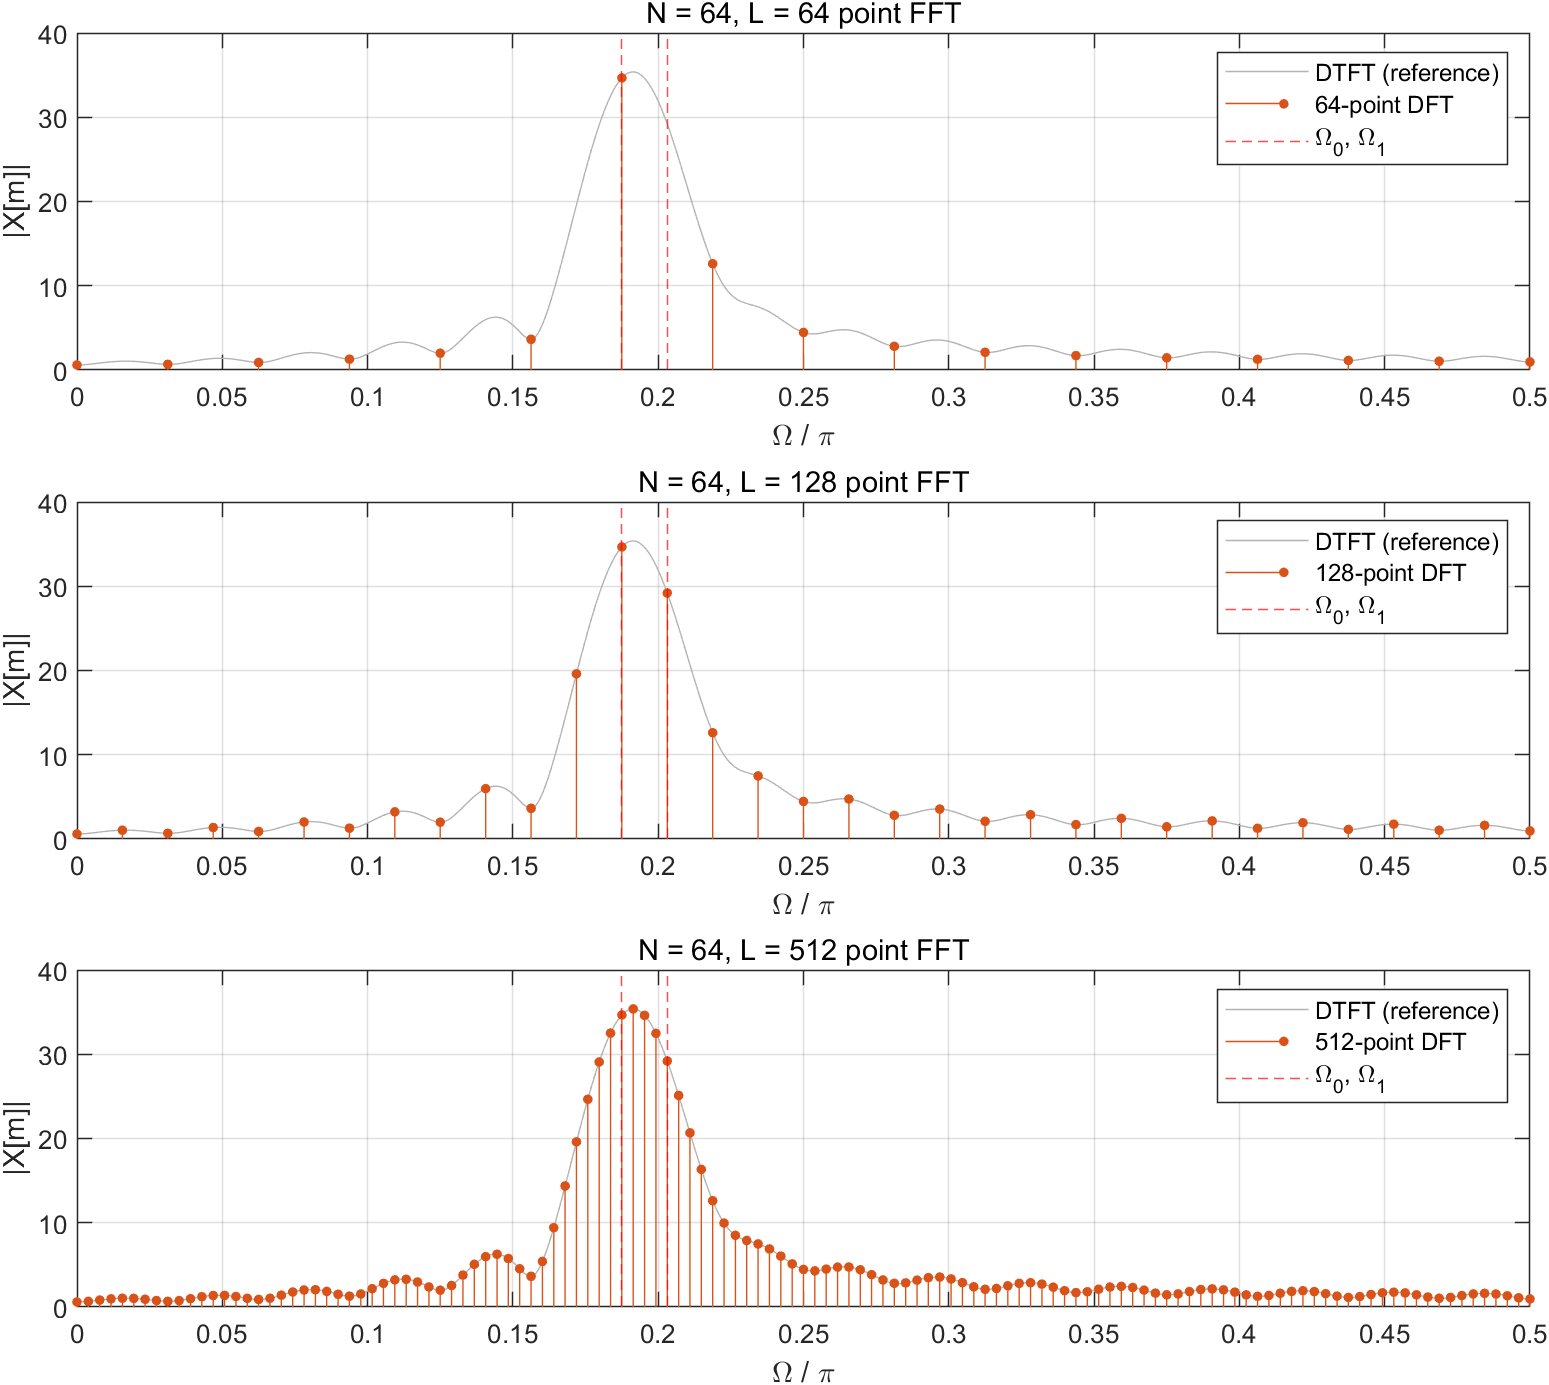
\includegraphics[width=0.78\textwidth]{Ex2_1_N64_zeropad.png}
    \caption{$N=64$ with $L=64$, $128$ and $512$. The grey curve is the DTFT of the 64-point record; the red dashed lines mark $\Omega_0$ and $\Omega_1$. Only one peak appears for every $L$.}
    \label{fig:ex2-1}
\end{figure}

\begin{figure}[!htbp]
    \centering
    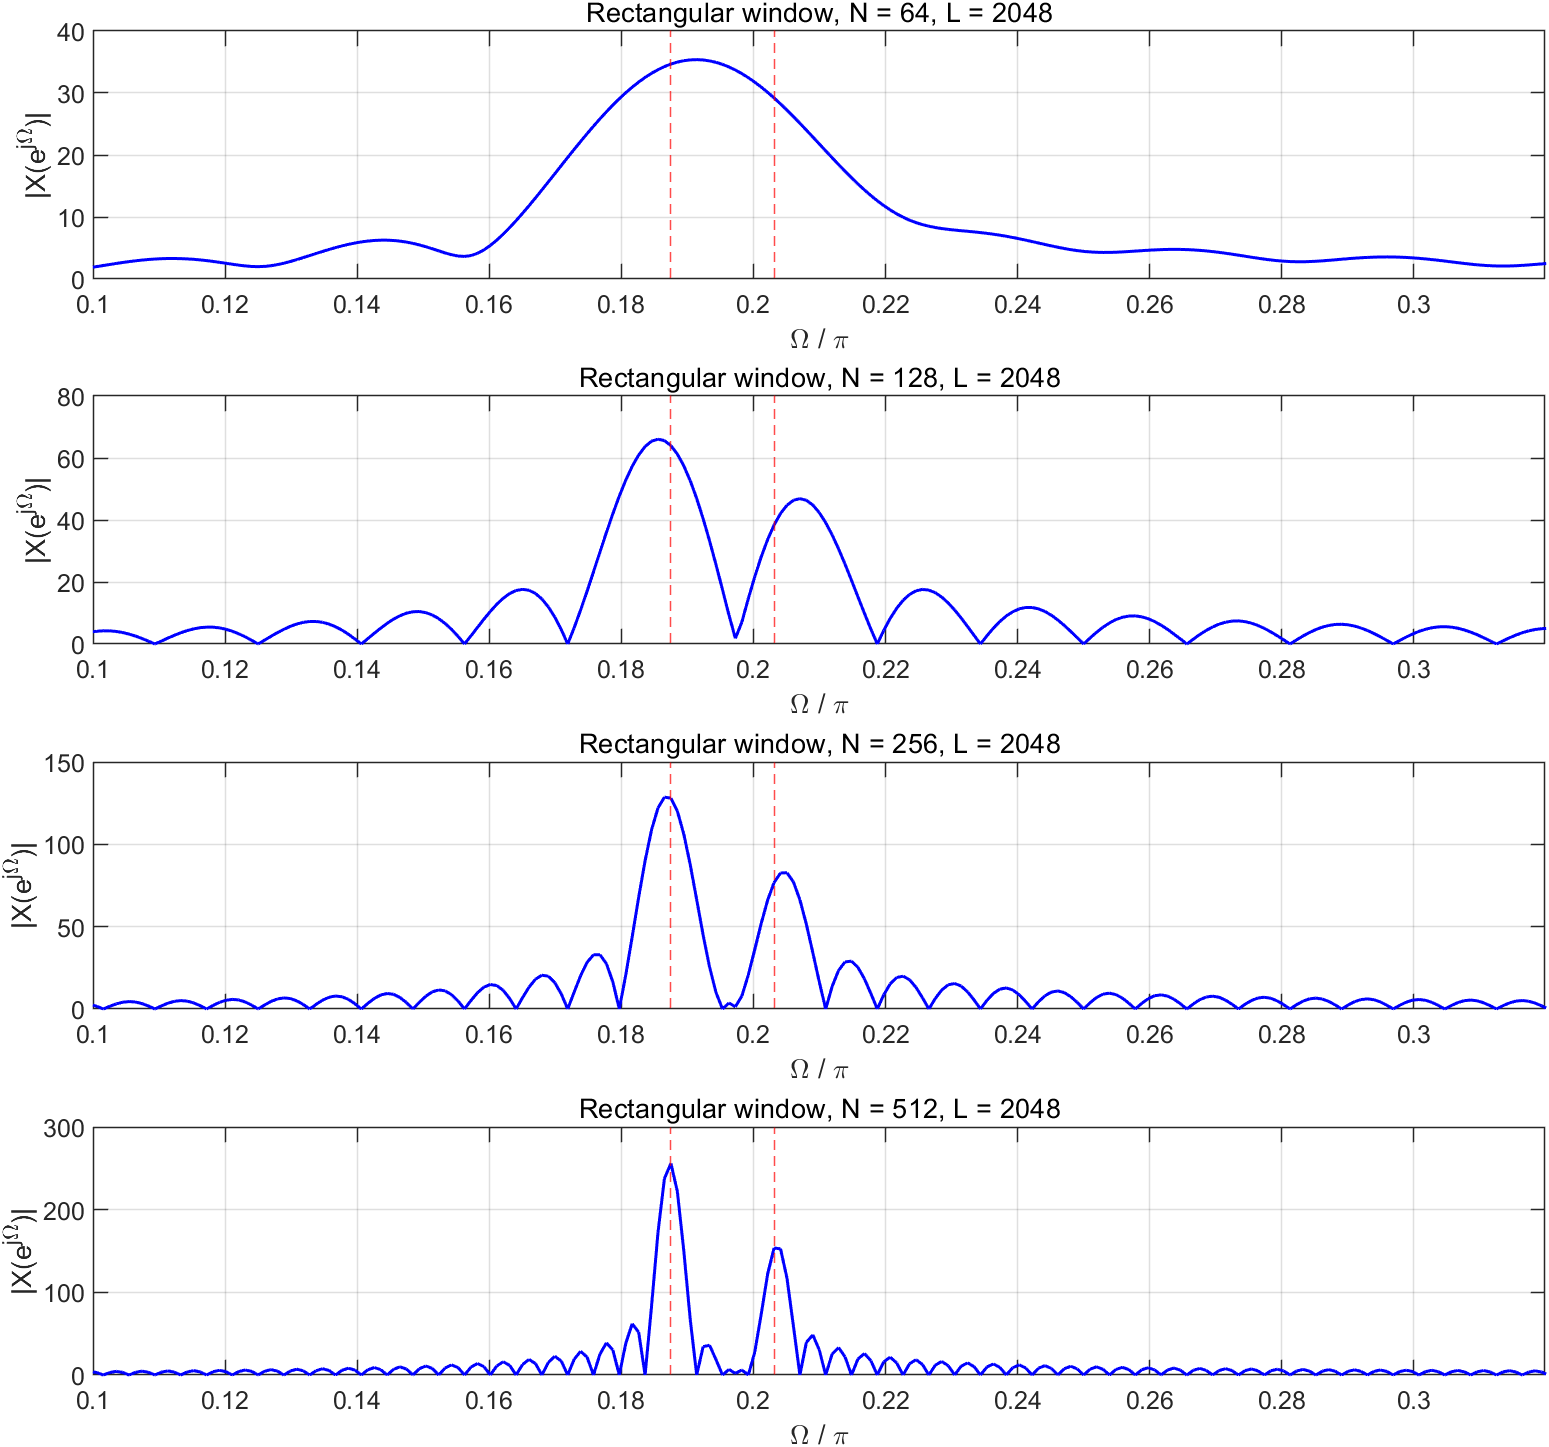
\includegraphics[width=0.85\textwidth]{Ex2_2_increaseN_rect.png}
    \caption{Rectangular window with increasing record length $N=64,128,256,512$ ($L=2048$). Two peaks appear from $N=128$ on.}
    \label{fig:ex2-2}
\end{figure}

\begin{figure}[!htbp]
    \centering
    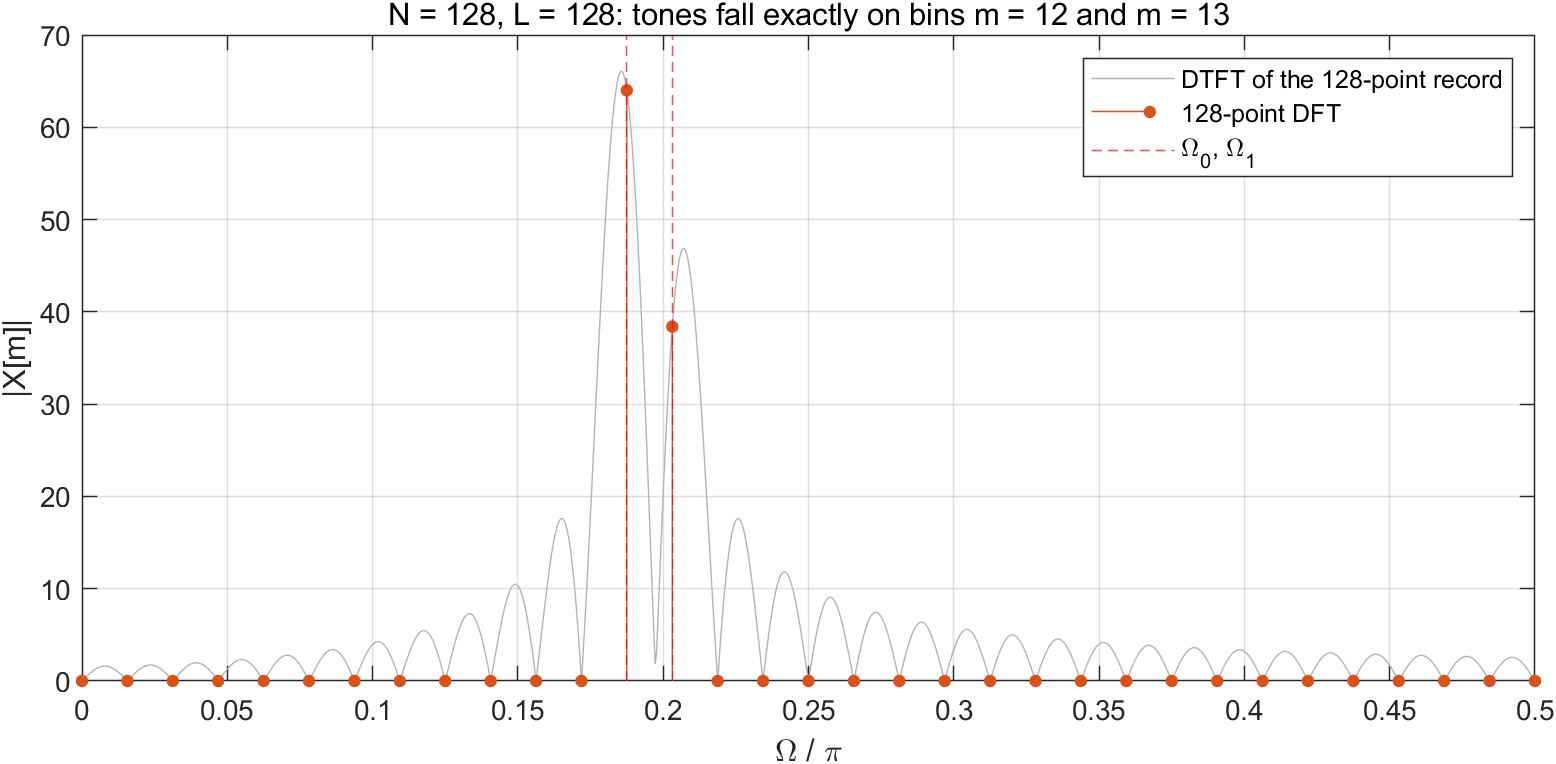
\includegraphics[width=1\textwidth]{Ex2_2a_N128_exactbins.png}
    \caption{The chosen parameters $N=L=128$: the 128-point DFT has only two non-zero bins, $m=12$ and $m=13$.}
    \label{fig:ex2-2a}
\end{figure}

\begin{figure}[!htbp]
    \centering
    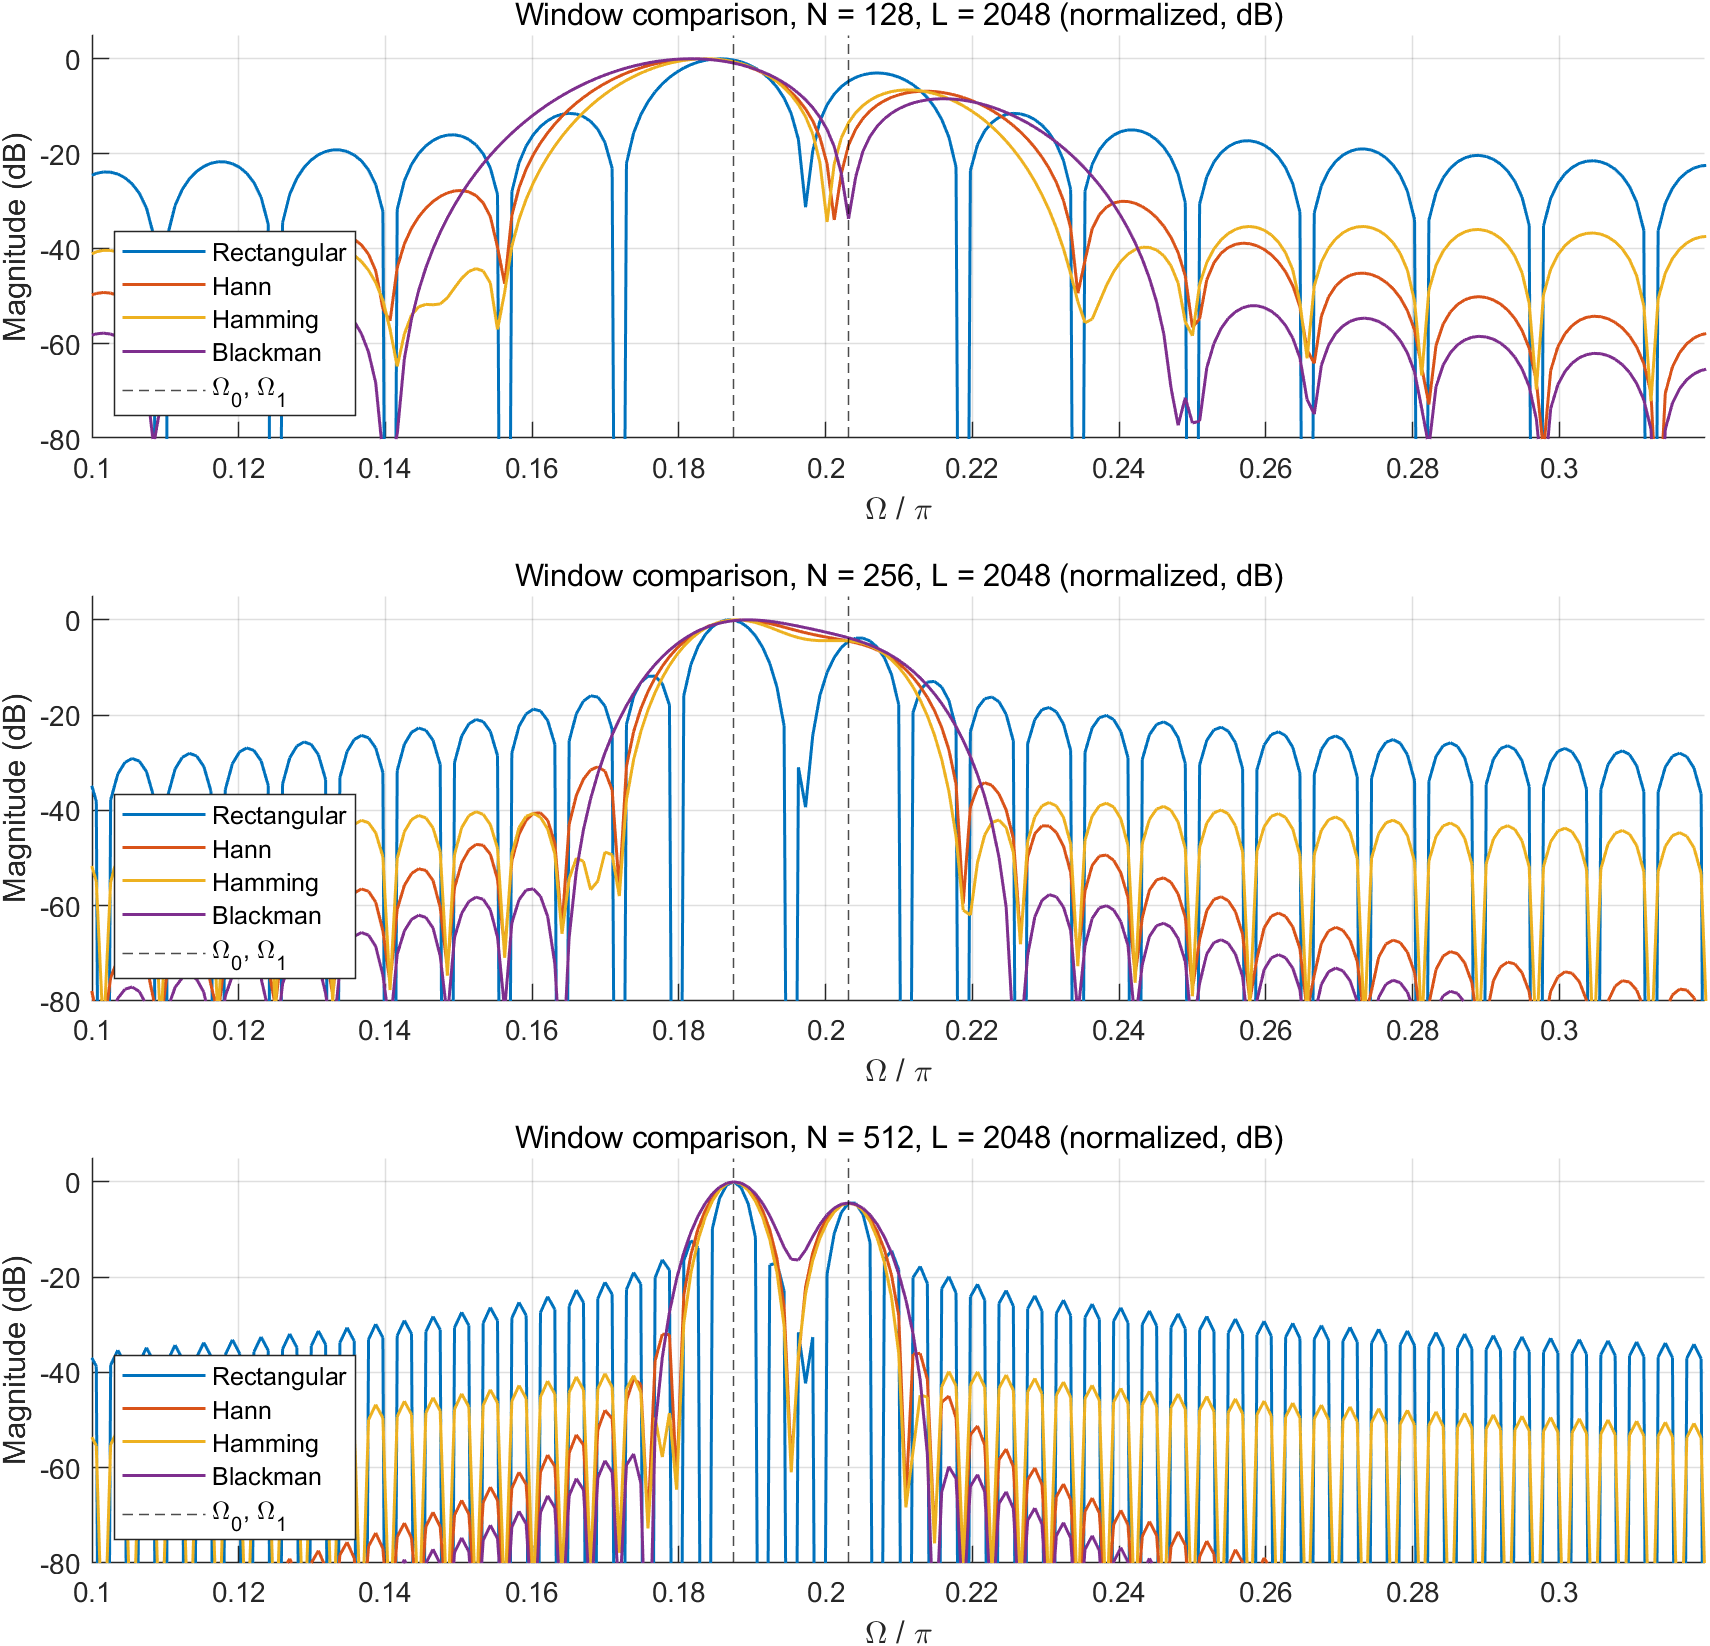
\includegraphics[width=0.75\textwidth]{Ex2_3_windows.png}
    \caption{Rectangular, Hann, Hamming and Blackman windows for $N=128$, $256$ and $512$ (normalised, dB).}
    \label{fig:ex2-3}
\end{figure}

\begin{table}[!htbp]
\centering
\caption{Detected peak positions $\Omega/\pi$ ($L=2048$). True values: $0.1875$ and $0.2031$.}
\label{tab:ex2}
\begin{tabular}{lccc}
\toprule
Window & $N=128$ & $N=256$ & $N=512$\\
\midrule
Rectangular & 0.1855, 0.2070 & 0.1865, 0.2051 & 0.1875, 0.2031\\
Hann        & 0.1826, 0.2139 & 0.1885 (one peak) & 0.1875, 0.2031\\
Hamming     & 0.1836, 0.2109 & 0.1875, 0.2021 & 0.1875, 0.2031\\
Blackman    & 0.1816, 0.2158 & 0.1895 (one peak) & 0.1875, 0.2031\\
\bottomrule
\end{tabular}
\end{table}

\subsection{Analysis of the Results}

\subsubsection{Zero Padding Does Not Improve Resolution}
Figure~\ref{fig:ex2-1} confirms the prediction. For $L=64$ the DFT samples happen to hit $\Omega_0$ (bin 6) exactly, but the second tone at bin 6.5 lies between two samples. For $L=128$ and $L=512$ the stems follow the grey DTFT curve more and more closely. That curve has a single broad peak near $0.19\pi$, so the peak counter finds one peak for all three values of $L$. Zero padding reduces the \emph{picket-fence effect} (we see the curve between the old bins) but adds no information. The resolution limit $2\pi/N$ is fixed by the 64 measured samples.

\subsubsection{Longer Records and the Best Choice of Parameters}
Figure~\ref{fig:ex2-2} shows that the record length is what matters. At $N=128$ the main lobes become narrow enough and a clear dip appears between two peaks. At $N=256$ and $512$ the peaks become sharper and move to the true positions: the peak-position error falls from $0.004\pi$ at $N=128$ to zero at $N=512$. The remaining bias at $N=128$ and $256$ comes from the tail of one main lobe adding to the other line.

Figure~\ref{fig:ex2-2a} shows the parameter set we propose for question (2): $N=L=128$. Because both tones complete an integer number of periods in the window, the DFT gives exactly $|X[12]|=64.00$ and $|X[13]|=38.40$. These values are $N/2$ and $0.6N/2$, so the amplitude ratio $0.6$ is recovered exactly. All other bins are below $5\times10^{-14}$, i.e.\ there is no leakage. This "coherent sampling" is the ideal case of DFT spectral analysis. It requires the frequencies to be known in advance; for unknown signals, $N\ge256$ with zero padding is the safer choice.

\subsubsection{Influence of the Window Type}
Figure~\ref{fig:ex2-3} and Table~\ref{tab:ex2} show the trade-off between main-lobe width and side-lobe level:
\begin{itemize}
    \item The \textbf{rectangular} window has the narrowest main lobe and is the only one that separates the lines at $N=128$ and $256$. Its side lobes are high ($-13$ dB), however; a weaker third component could be hidden under them.
    \item \textbf{Hann, Hamming and Blackman} suppress the side lobes to $-31$, $-41$ and $-57$ dB, but their wider main lobes merge the two lines at $N=256$ for Hann and Blackman. Hamming only just separates them, with a biased second peak. All windows give correct results at $N=512$, as the minimum lengths in Table~\ref{tab:windows} predict.
    \item An important pitfall appears at $N=128$: all tapered windows show \emph{two} peaks, but at clearly wrong positions (for example, Blackman at $0.1816\pi$ and $0.2158\pi$). Because the two lobes overlap and add as complex numbers with different phases, a dip appears between them. These are not resolved lines. Counting peaks alone is therefore not enough; the peak positions must also be checked against the theoretical resolution.
\end{itemize}

In summary, the record length $N$ (i.e.\ the observation time) determines the resolution. The DFT length $L$ determines only how densely the spectrum is sampled. The window type trades resolution against leakage: for close lines of similar amplitude the rectangular window is best, while for lines of very different amplitude a low-side-lobe window together with a longer $N$ is needed.

% =====================================================================
\section{Topic 3: Spectrum of the Scale Signal and Its Key}

\subsection{Analysis of the Simulation Task}

\textbf{Signal parameters.} \texttt{audioread} returns $f_s=8000$ Hz and $N=32000$ samples (mono, 16 bit), so the duration is
\begin{equation}
    T=\frac{N}{f_s}=\frac{32000}{8000}=4\ \text{s}.
\end{equation}

\textbf{Choice of the DFT length.} The closest notes of the scale are E4 and F4, $349.23-329.63=19.6$ Hz apart. The whole record gives a resolution of $1/T=0.25$ Hz, far finer than needed. We use $L=2^{\lceil\log_2N\rceil}=32768\ge N$, which gives a bin spacing of $f_s/L=0.244$ Hz, so the FFT is efficient and no data are lost. The useful band is $0$--$f_s/2=4000$ Hz.

\textbf{Determining the key.} The DFT of the whole record tells us \emph{which} frequencies are present, not \emph{when}. To find the order of the notes we also use a short-time analysis (spectrogram) and an automatic segmentation:
\begin{enumerate}
    \item Frames of 512 samples (64 ms) with a hop of 128 samples are Hann-windowed. The dominant frequency of each frame is rounded to the nearest semitone.
    \item A new note starts whenever this semitone changes. Each boundary is then moved to the minimum of the short-time energy within $\pm40$ ms, because the notes fade to silence at their boundaries.
    \item Every note is analysed separately: Hann window, 8192-point DFT, and parabolic interpolation of the peak \cite{smith} for sub-bin accuracy. Each note lasts 0.5 s, so the resolution is about 2 Hz, still well below 19.6 Hz.
\end{enumerate}
The semitone steps between consecutive notes reveal the scale type. A major scale has the pattern whole--whole--half--whole--whole--whole--half (2 2 1 2 2 2 1). Its first note (``do'', 1) names the key \cite{chen}.

\subsection{Simulation Code}

\begin{lstlisting}[caption={Topic 3: parameters, whole-record DFT, per-note analysis and key detection (excerpt of \texttt{ex3\_scale.m})}]
[x, fs] = audioread('yueyin1.wav');
N = length(x);  T = N/fs;                 % 32000 samples, 4 s
L = 2^nextpow2(N);                        % 32768-point DFT
X = abs(fft(x, L)) / N * 2;               % single-sided amplitude
f = (0:L-1) * fs / L;
[pk, loc] = findpeaks(X(1:L/2), 'MinPeakHeight', 0.2*max(X), ...
                      'MinPeakDistance', round(10/(fs/L)));
spectrogram(x, hann(1024), 768, 4096, fs, 'yaxis');   % note order

seg = segmentNotes(x, fs);                % pitch-change segmentation
for k = 1:size(seg,1)
    xs = x(seg(k,1):seg(k,2));
    Xs = abs(fft(xs .* hann(numel(xs)), 8192));
    [~, im] = max(Xs(1:4096));
    f0(k) = parabolicPeak(Xs, im) * fs / 8192;     % sub-bin peak
    midi(k) = round(69 + 12*log2(f0(k)/440));      % nearest note
end
steps = diff(midi);                       % [2 2 1 2 2 2 1] -> major
\end{lstlisting}

\subsection{Simulation Results}

\begin{figure}[!htbp]
    \centering
    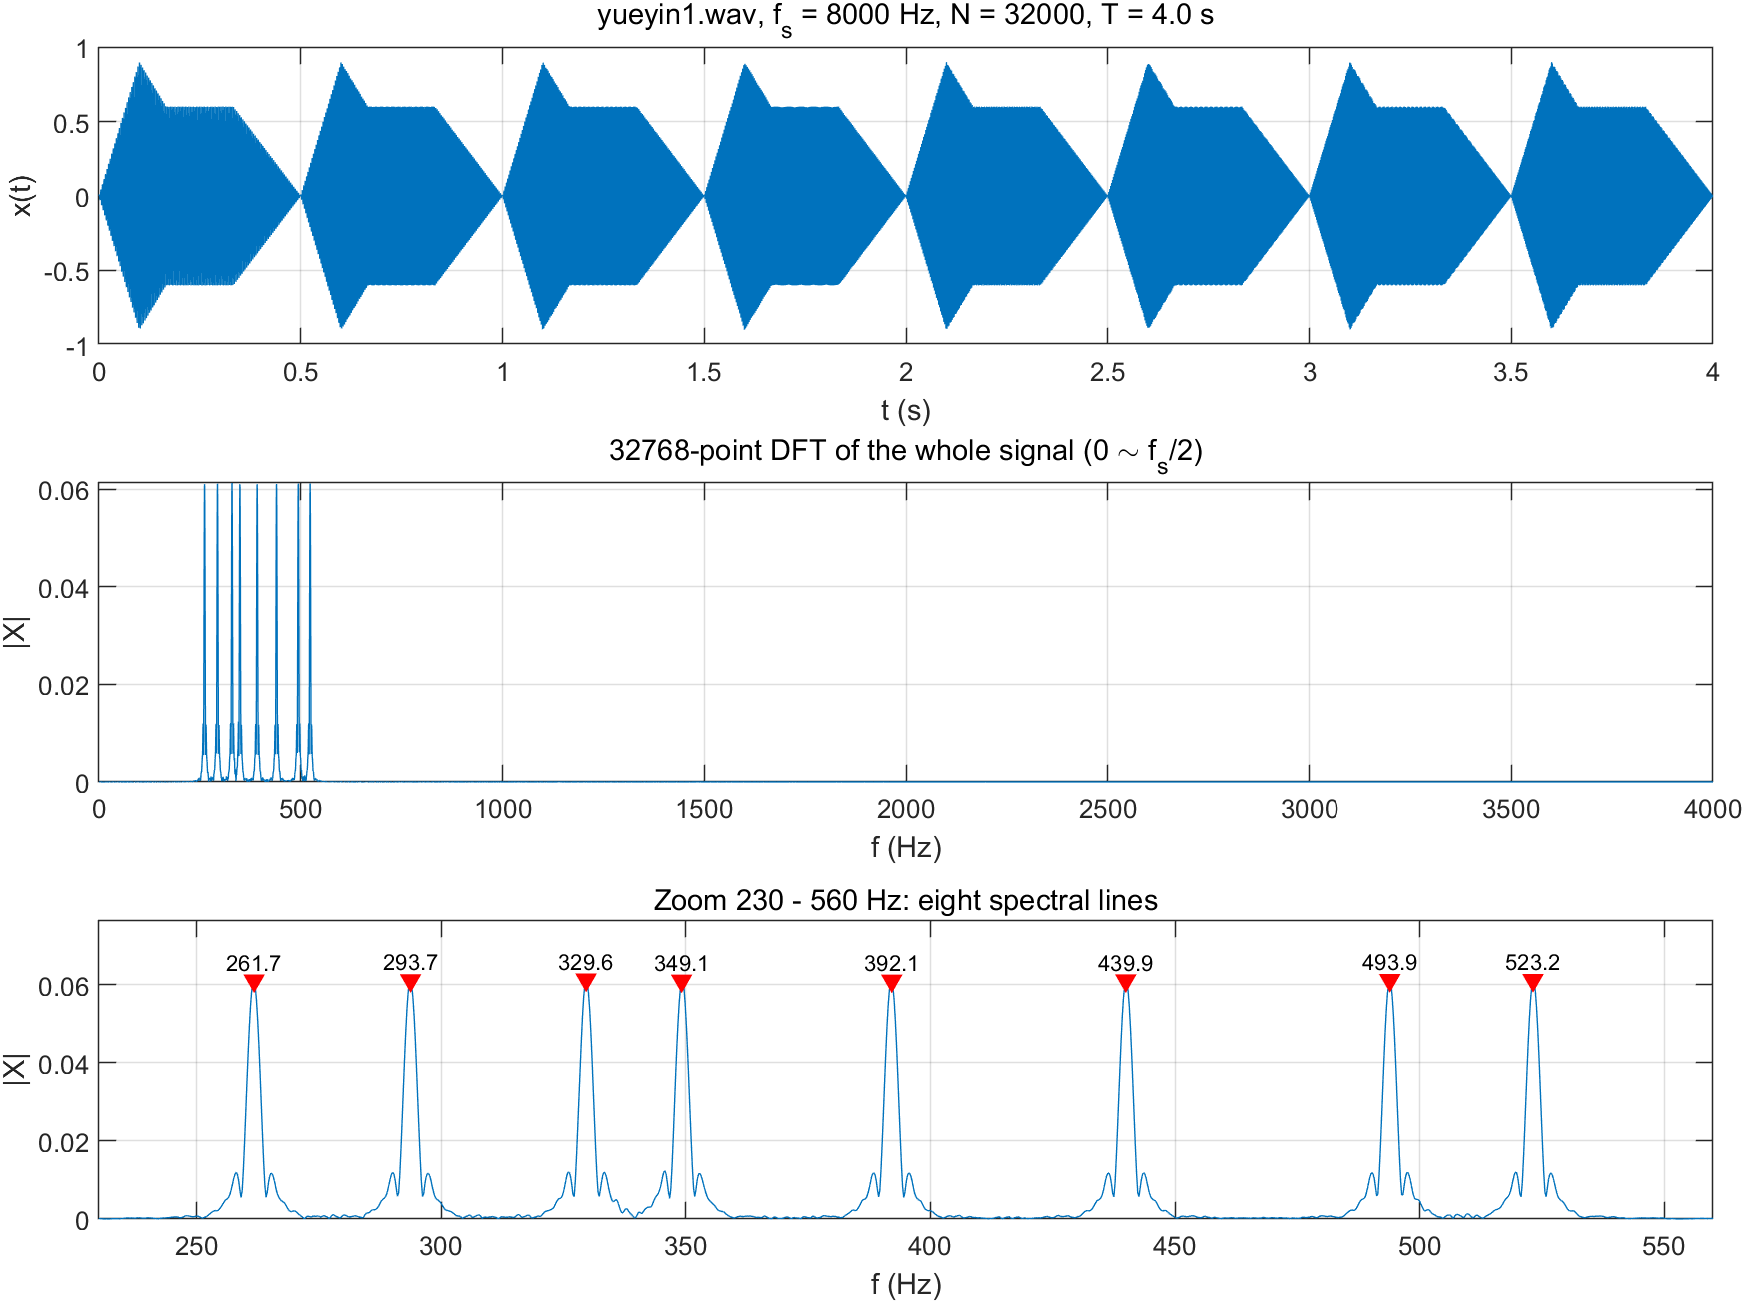
\includegraphics[width=0.94\textwidth]{Ex3_1_whole_spectrum.png}
    \caption{\texttt{yueyin1.wav}: waveform (top), 32768-point DFT over $0$--$f_s/2$ (middle), and zoom on $230$--$560$ Hz with the eight detected lines (bottom).}
    \label{fig:ex3-1}
\end{figure}

\begin{figure}[!htbp]
    \centering
    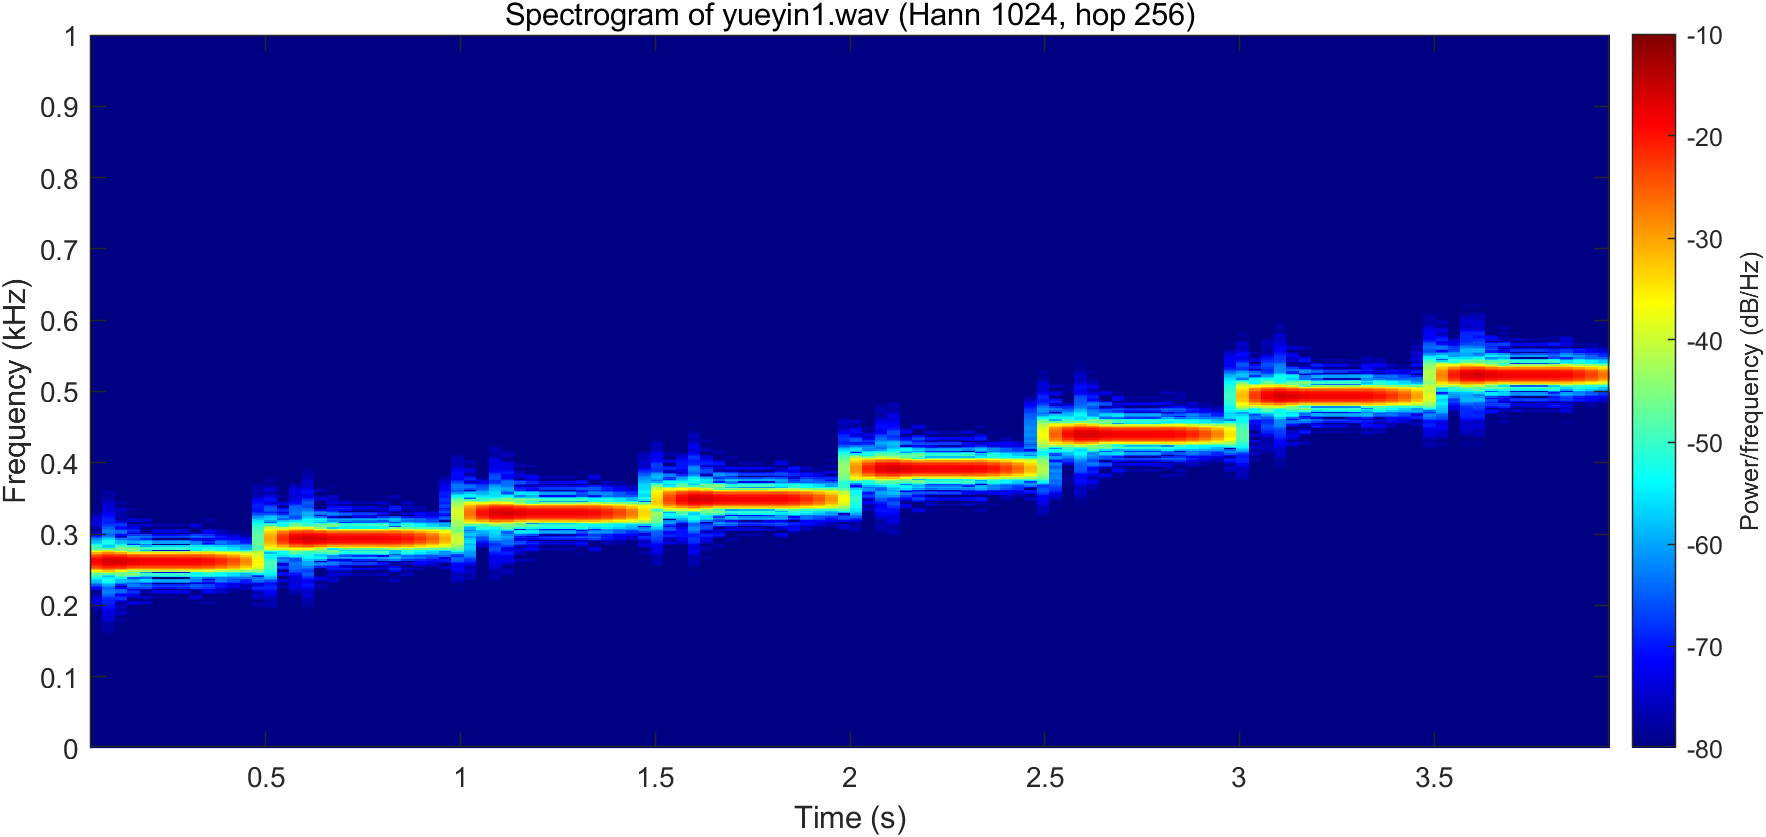
\includegraphics[width=1\textwidth]{Ex3_2_spectrogram.png}
    \caption{Spectrogram (Hann window of 1024 samples, hop 256): eight notes rising in pitch, each lasting 0.5 s.}
    \label{fig:ex3-2}
\end{figure}

\begin{figure}[!htbp]
    \centering
    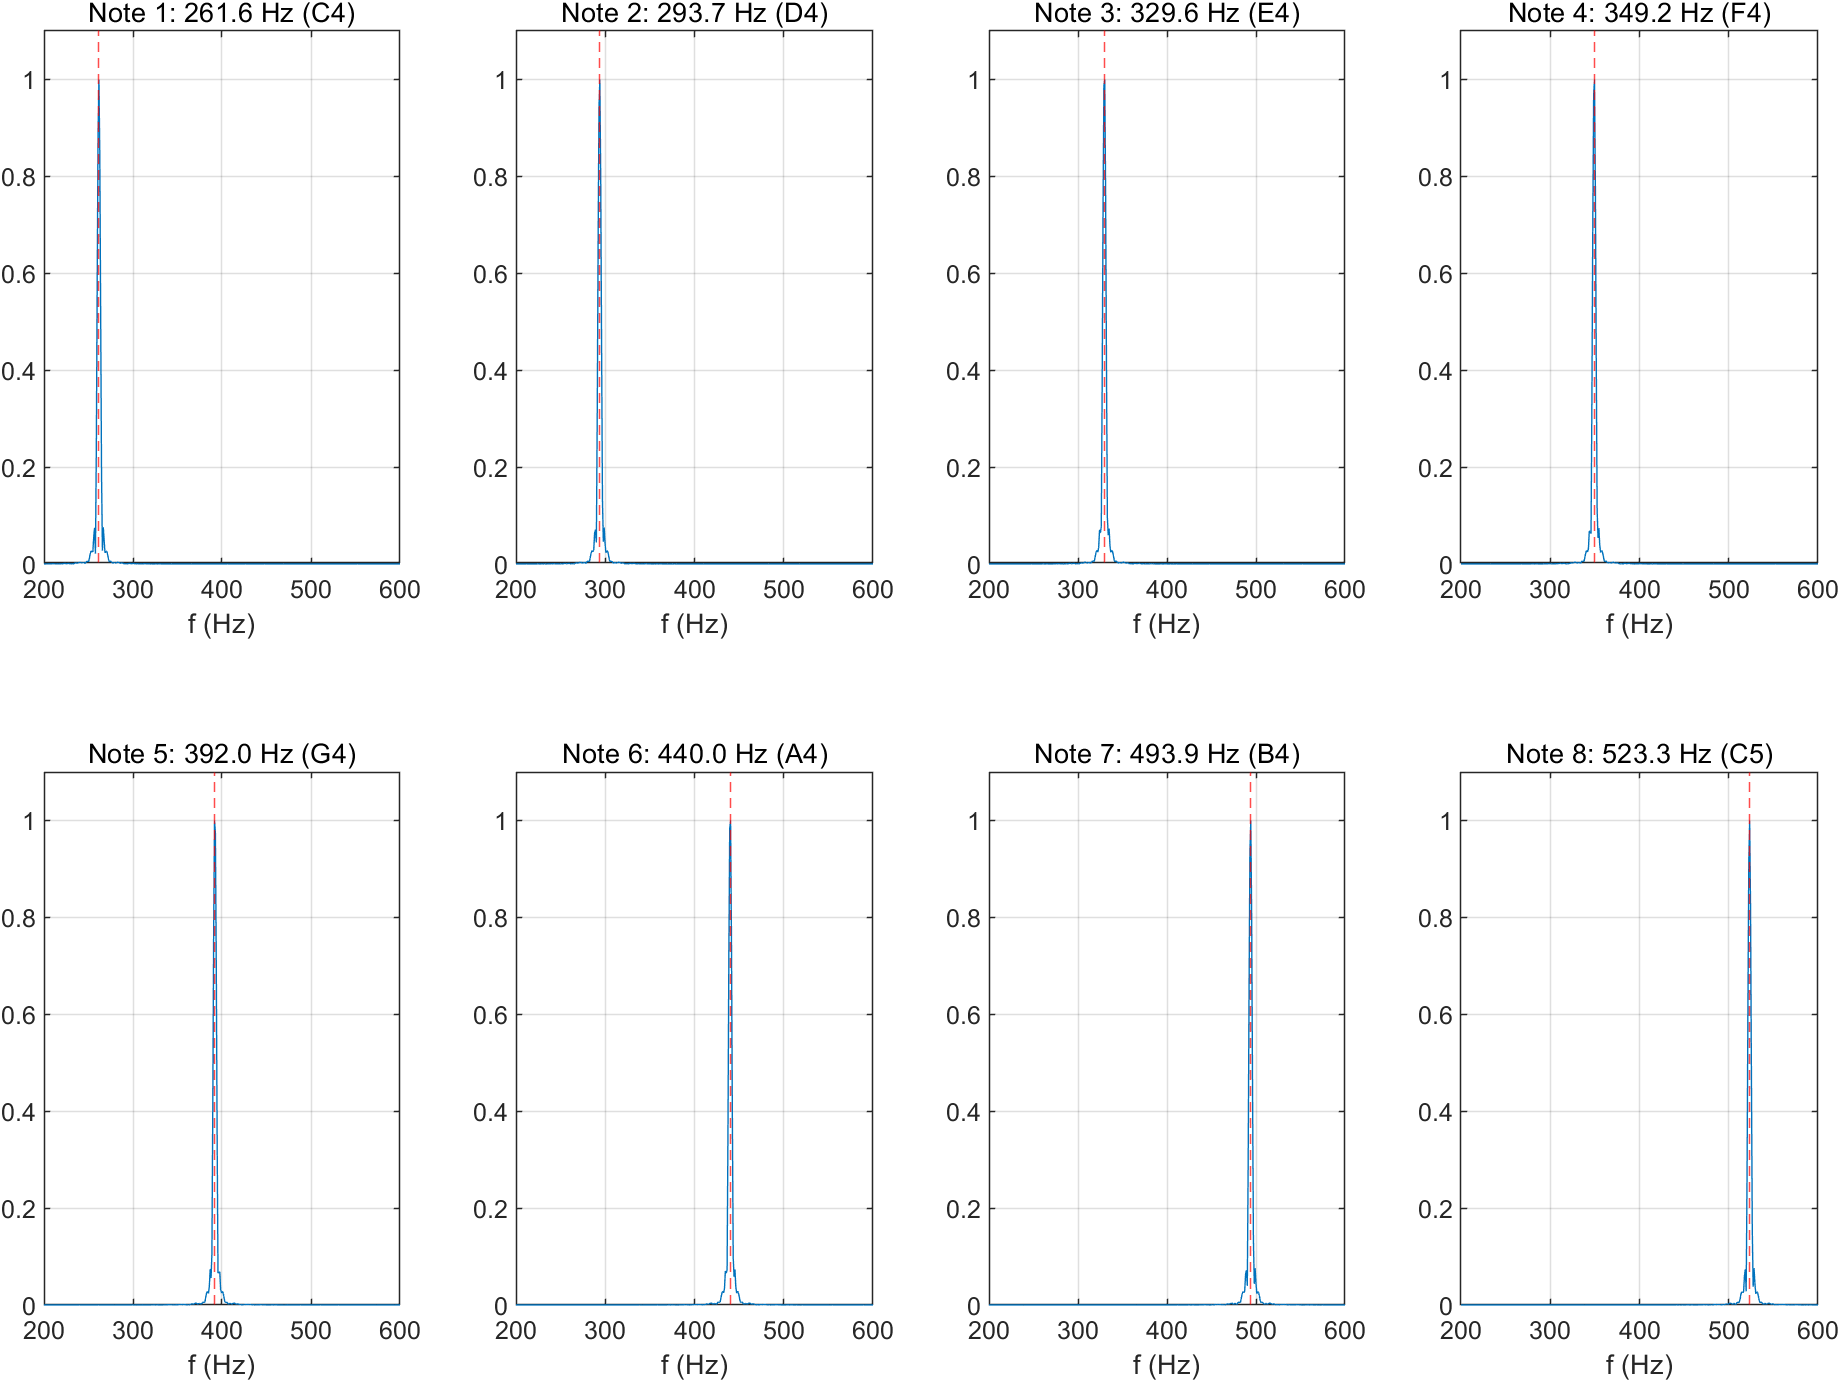
\includegraphics[width=1\textwidth]{Ex3_3_per_note_spectra.png}
    \caption{DFT of every individual note (Hann window, $L=8192$) with the estimated pitch.}
    \label{fig:ex3-3}
\end{figure}

\begin{figure}[!htbp]
    \centering
    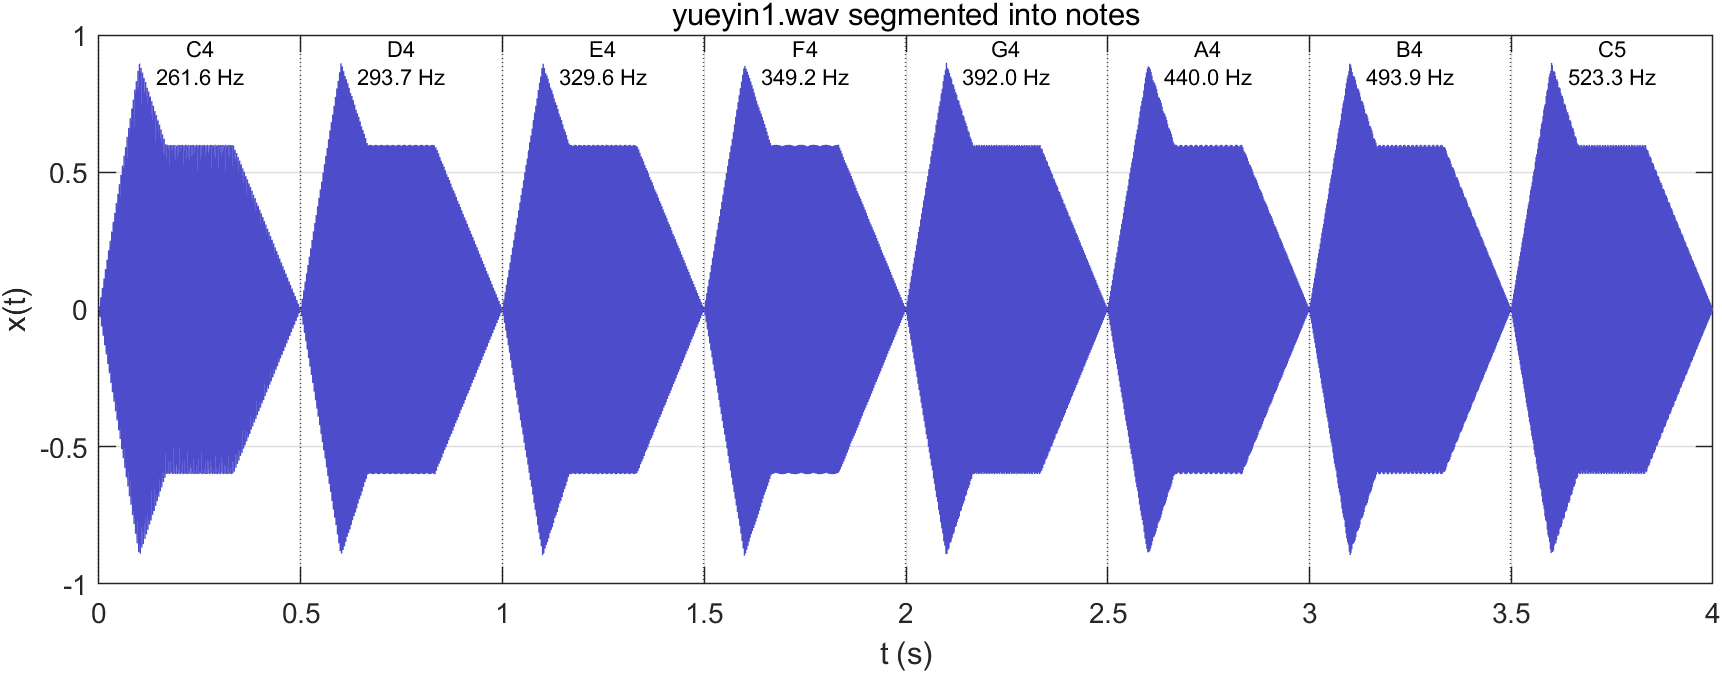
\includegraphics[width=0.95\textwidth]{Ex3_4_waveform_notes.png}
    \caption{Waveform with the automatically detected note boundaries and pitches.}
    \label{fig:ex3-4}
\end{figure}

\begin{table}[!htbp]
\centering
\caption{Measured pitches of \texttt{yueyin1.wav} compared with the C-major table.}
\label{tab:ex3}
\begin{tabular}{cccccc}
\toprule
Note & Time (s) & Measured (Hz) & Note name & Table (Hz) & Error (Hz)\\
\midrule
1 & 0.0--0.5 & 261.63 & C4 & 261.63 & $+0.00$\\
2 & 0.5--1.0 & 293.67 & D4 & 293.66 & $+0.01$\\
3 & 1.0--1.5 & 329.63 & E4 & 329.63 & $+0.00$\\
4 & 1.5--2.0 & 349.24 & F4 & 349.23 & $+0.01$\\
5 & 2.0--2.5 & 391.99 & G4 & 392.00 & $-0.01$\\
6 & 2.5--3.0 & 440.01 & A4 & 440.00 & $+0.01$\\
7 & 3.0--3.5 & 493.89 & B4 & 493.88 & $+0.01$\\
$\dot{1}$ & 3.5--4.0 & 523.26 & C5 & 523.25 & $+0.01$\\
\bottomrule
\end{tabular}
\end{table}

\subsection{Analysis of the Results}

\subsubsection{Whole-Record Spectrum}
Figure~\ref{fig:ex3-1} shows that all energy is concentrated between 260 and 530 Hz. Above that band there is nothing, so the signal consists of pure tones without harmonics. The zoom reveals exactly eight lines, at 261.7, 293.7, 329.6, 349.1, 392.1, 439.9, 493.9 and 523.2 Hz, each within one cent of an equal-tempered note. All lines have the same height ($\approx0.061$), because every note has the same amplitude envelope and occupies $1/8$ of the record.

Each line has small side lines a few hertz (about $\pm5$ Hz) away. They are not extra notes. Every note is switched on and off with an attack/decay envelope of length 0.5 s (top of Figure~\ref{fig:ex3-1}), and the spectrum of this envelope, whose features scale with $1/(0.5\ \text{s})=2$ Hz, is convolved with each line. This is the leakage effect of the "natural" window created by the note duration.

\subsubsection{Order of the Notes and the Key}
The whole-record DFT cannot tell the order in which the notes are played. The spectrogram (Figure~\ref{fig:ex3-2}) adds the time information: it shows an ascending staircase of eight 0.5 s steps. The automatic segmentation finds note boundaries at 0.499, 0.999, \dots, 3.499 s, i.e.\ exactly every 0.5 s (Figure~\ref{fig:ex3-4}). The per-note DFTs (Figure~\ref{fig:ex3-3}) give pitches that agree with the table within $\pm0.01$ Hz (Table~\ref{tab:ex3}).

The notes are C4, D4, E4, F4, G4, A4, B4, C5, with semitone steps $[2,2,1,2,2,2,1]$. This is the major-scale pattern, starting and ending on C. The signal is therefore an ascending \textbf{C major scale (1 = C)}, from middle C (C4, 261.63 Hz) to C5 (523.25 Hz), whose frequency ratio is exactly $2{:}1$ (one octave).

% =====================================================================
\section{Topic 4: Spectral Components of a Chord}

\subsection{Analysis of the Simulation Task}

\textbf{For question (1)}, \texttt{hexian1.wav} has $f_s=8000$ Hz and $N=8000$ samples ($T=1$ s), so the resolution is $1/T=1$ Hz. Neighbouring notes are at least one semitone, i.e.\ $\ge15$ Hz, apart in this range, so the DFT of the whole record easily separates the components of $x(t)=\sum_{i=1}^{3}\cos(2\pi f_it)$. We use $L=32768$ (zero padding) to read the peaks accurately and convert each peak to a note name.

\textbf{For question (2)}, a whole note lasts 0.2 s, so a 16th note lasts
\begin{equation}
    T_{16}=\frac{0.2}{16}=12.5\ \text{ms}\quad\Longrightarrow\quad N_{16}=T_{16}f_s=100\ \text{samples}.
\end{equation}
The best possible resolution is then $f_s/N_{16}=1/T_{16}=80$ Hz. The rectangular window's main lobe spans $\pm80$ Hz, and a Hann window's spans $\pm160$ Hz. In the chord found in (1), the notes are only $369.99-293.66=76.3$ Hz and $440-369.99=70.0$ Hz apart, \emph{smaller} than the resolution. We therefore predict:
\begin{itemize}
    \item The three main lobes overlap, so the DFT cannot resolve the notes. At best it shows distorted bumps at wrong frequencies, which can easily be mistaken for neighbouring semitones (the semitone spacing here is only 17--26 Hz).
    \item Zero padding cannot help, since it adds no information. A tapered window makes the problem worse.
    \item To resolve 70 Hz we need $T\ge1/70\approx14.3$ ms with a rectangular window and $T\ge2/70\approx28.6$ ms with a Hann window, i.e.\ at least an 8th note ($25$ ms) or better a quarter note ($50$ ms).
\end{itemize}

\textbf{Experiment design.} The 16th note is obtained by cutting the first $N=100$ samples of \texttt{hexian1.wav}. For comparison, we also analyse records of 1/8, 1/4, 1/2 and whole-note duration (200, 400, 800, 1600 samples) with rectangular and Hann windows. To show that the problem is general, we repeat the 16th-note test on a synthesised C-major chord (C4--E4--G4).

\textbf{A remedy.} The DFT fails because it assumes nothing about the signal. Musical notes, however, can only take the discrete frequencies $f(m)$ of the equal-tempered scale. Using this prior knowledge, we fit the model
\begin{equation}
    x[n]\approx\sum_{i=1}^{3}\Big[a_i\cos\!\Big(\frac{2\pi f(m_i)n}{f_s}\Big)+b_i\sin\!\Big(\frac{2\pi f(m_i)n}{f_s}\Big)\Big]=\boldsymbol{\Phi}\mathbf{c}
\end{equation}
by least squares, $\mathbf{c}=\boldsymbol{\Phi}^{+}\mathbf{x}$, for every set of three candidate notes from C4 to B5 ($\binom{24}{3}=2024$ sets). We keep the set with the smallest relative residual $\|\mathbf{x}-\boldsymbol{\Phi}\mathbf{c}\|^2/\|\mathbf{x}\|^2$. This parametric approach is not limited by the $1/T$ resolution of the DFT \cite{stoica}.

\subsection{Simulation Code}

\begin{lstlisting}[caption={Topic 4: chord analysis, short-note experiment and least-squares note fit (excerpt of \texttt{ex4\_chord.m})}]
[x, fs] = audioread('hexian1.wav');           % 8000 samples, 1 s
L = 4 * 2^nextpow2(length(x));
X = abs(fft(x, L)) / length(x) * 2;
[pk, loc] = findpeaks(X(1:L/2), 'MinPeakHeight', 0.3*max(X));
fChord = (loc-1) * fs / L;                     % -> D4, F#4, A4

% (2) 1/16, 1/8, 1/4, 1/2 and whole note (whole note = 0.2 s)
durs = 0.2 ./ [16 8 4 2 1];
for i = 1:numel(durs)
    Ns = round(durs(i)*fs);   xs = x(1:Ns);   % 16th note: 100 samples
    Xr = abs(fft(xs, 8192));                   % rectangular window
    Xh = abs(fft(xs .* hann(Ns), 8192));       % Hann window
end

% Remedy: least-squares fit on the equal-tempered note grid
function [bestSet, bestRes] = lsChordFit(x, fs, cand, K)
n = (0:numel(x)-1).';   bestRes = inf;
combos = nchoosek(cand, K);                    % all K-note combinations
for i = 1:size(combos, 1)
    fk = 440 * 2.^((combos(i,:) - 69)/12);
    A  = [cos(2*pi*n*fk/fs), sin(2*pi*n*fk/fs)];
    c  = A \ x(:);                             % least squares
    r  = norm(x(:) - A*c)^2 / norm(x)^2;
    if r < bestRes, bestRes = r; bestSet = combos(i,:); end
end
end
\end{lstlisting}

\subsection{Simulation Results}

\begin{figure}[!htbp]
    \centering
    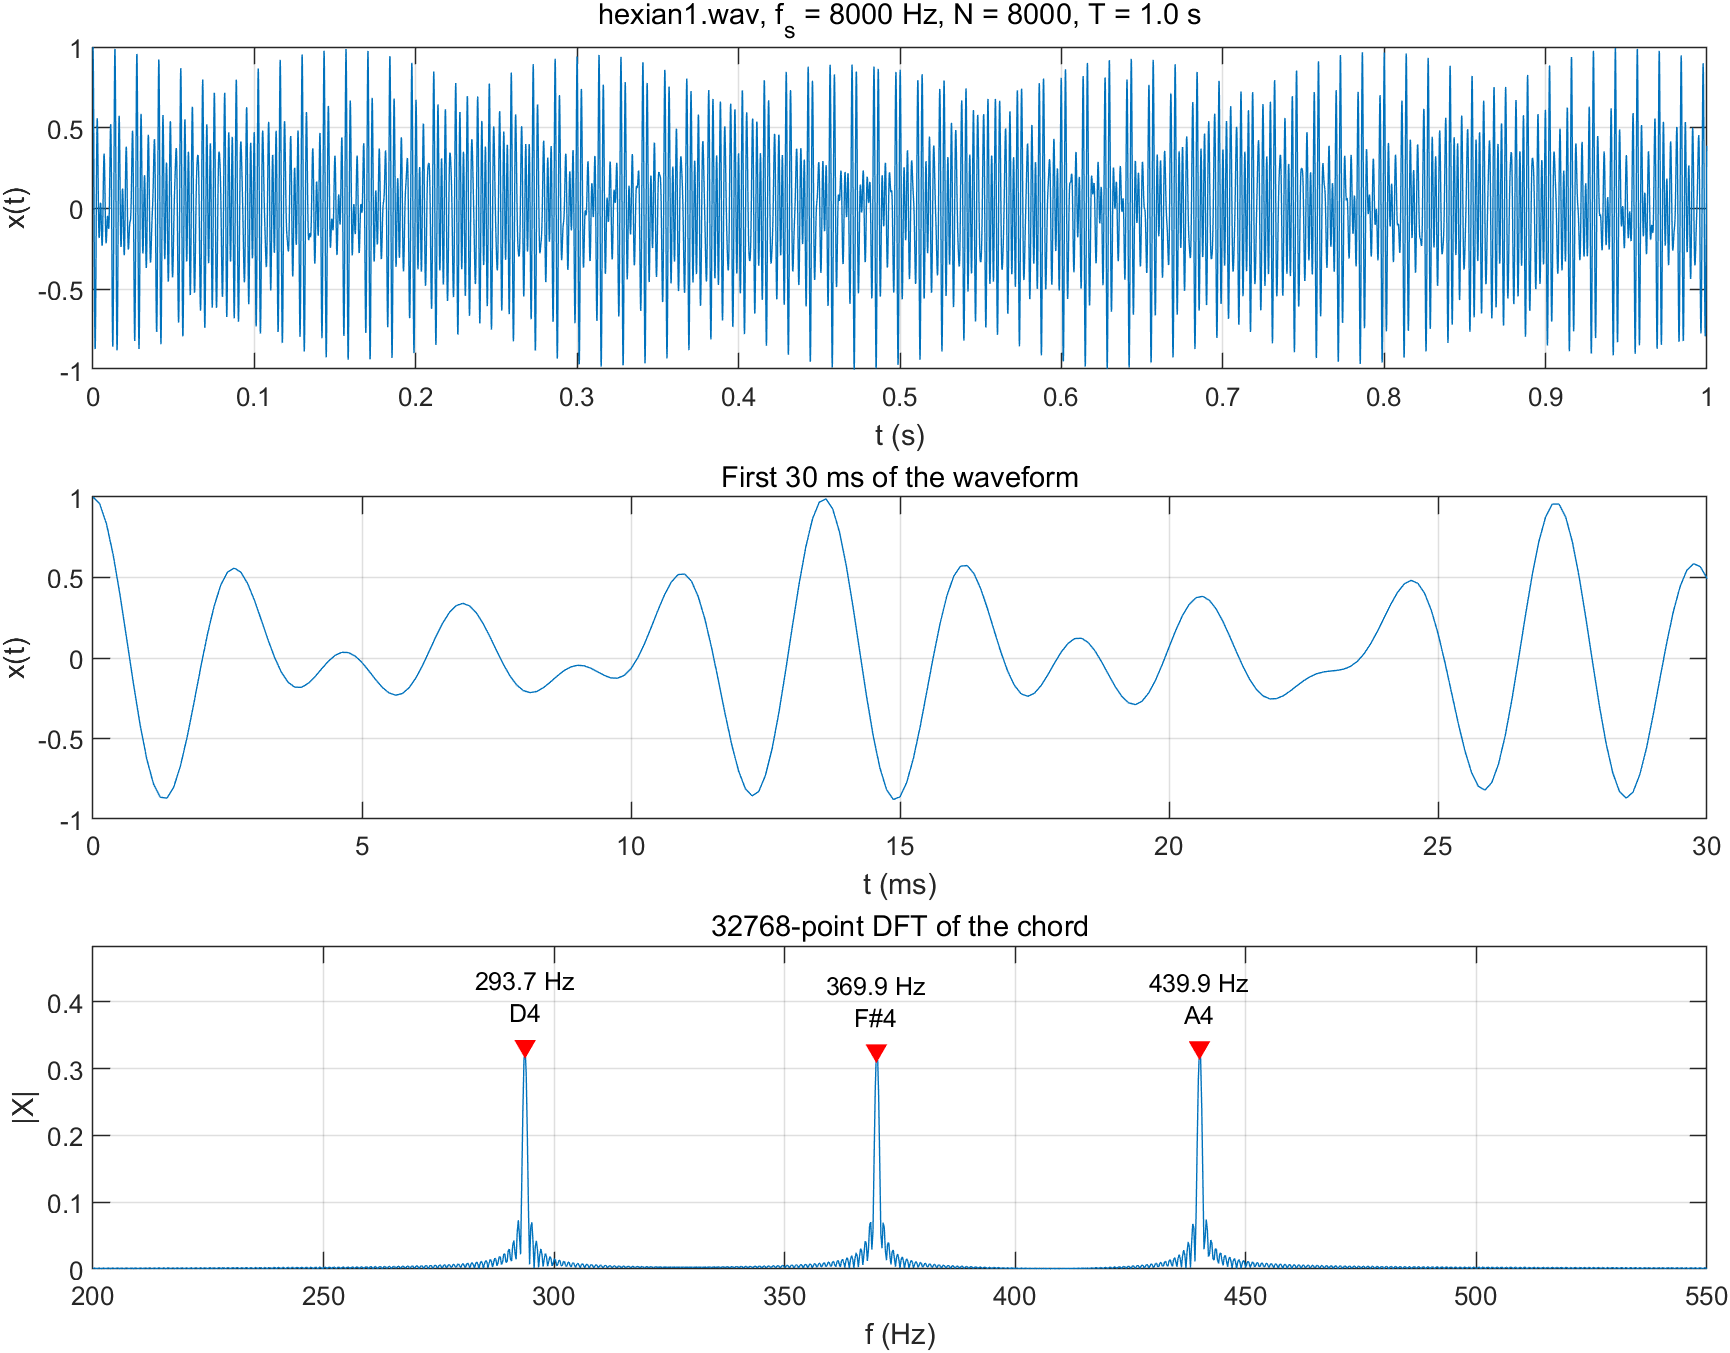
\includegraphics[width=0.82\textwidth]{Ex4_1_chord_spectrum.png}
    \caption{\texttt{hexian1.wav}: full waveform, first 30 ms, and DFT with the three detected components.}
    \label{fig:ex4-1}
\end{figure}

\begin{figure}[!htbp]
    \centering
    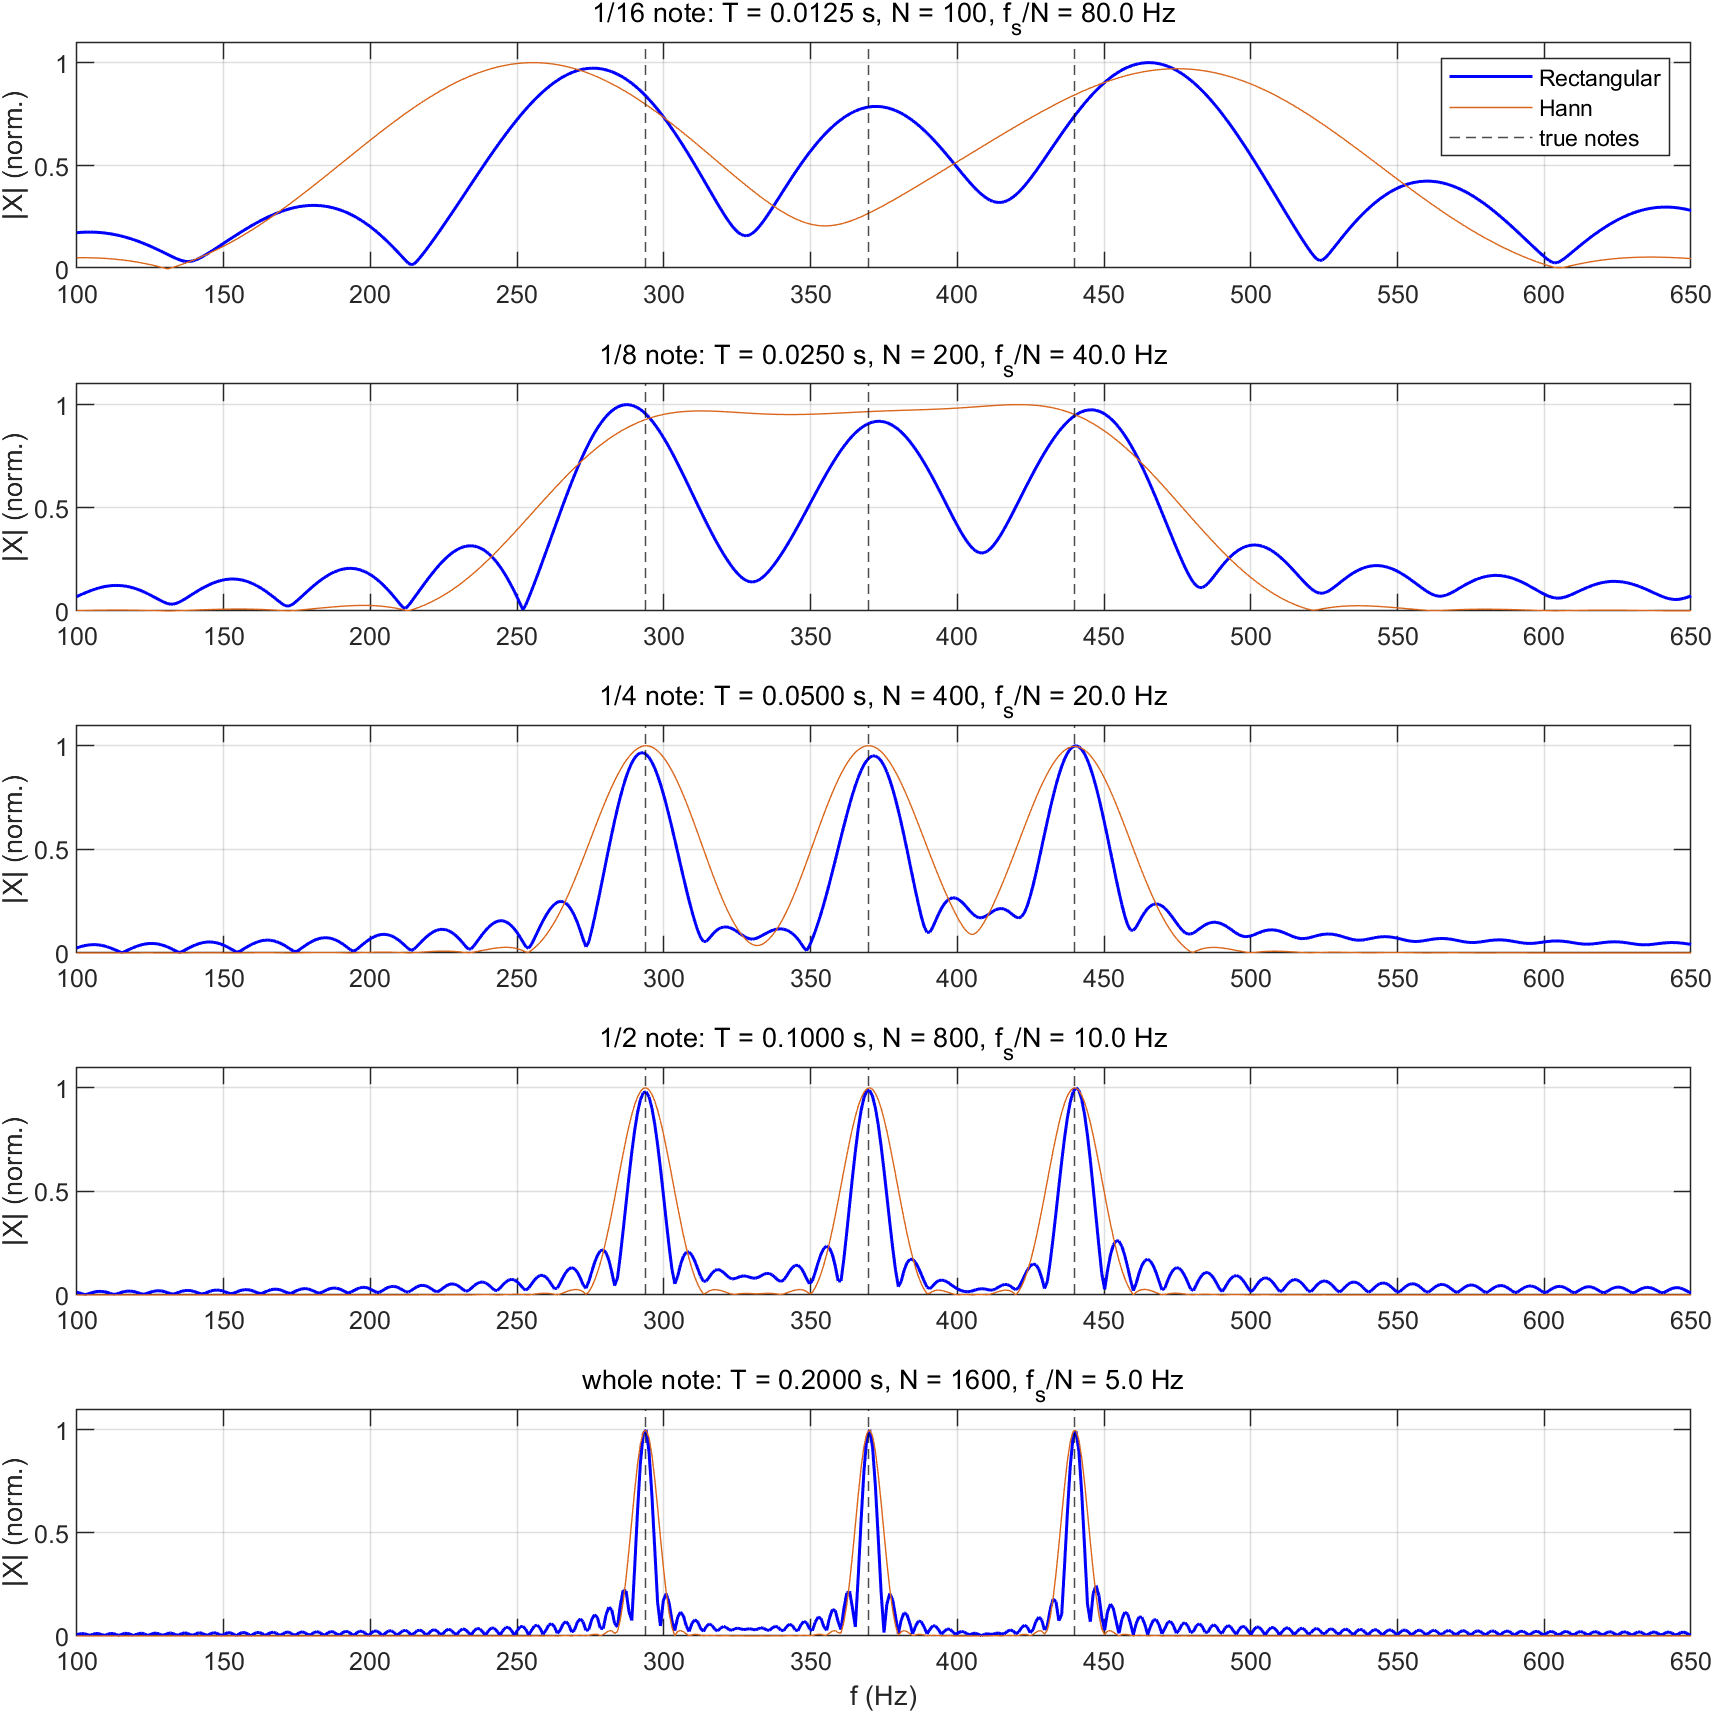
\includegraphics[width=0.75\textwidth]{Ex4_2_duration_vs_resolution.png}
    \caption{Spectrum of the chord for records of 1/16, 1/8, 1/4, 1/2 and whole-note duration (blue: rectangular, orange: Hann; dashed: true notes).}
    \label{fig:ex4-2}
\end{figure}

\begin{figure}[!htbp]
    \centering
    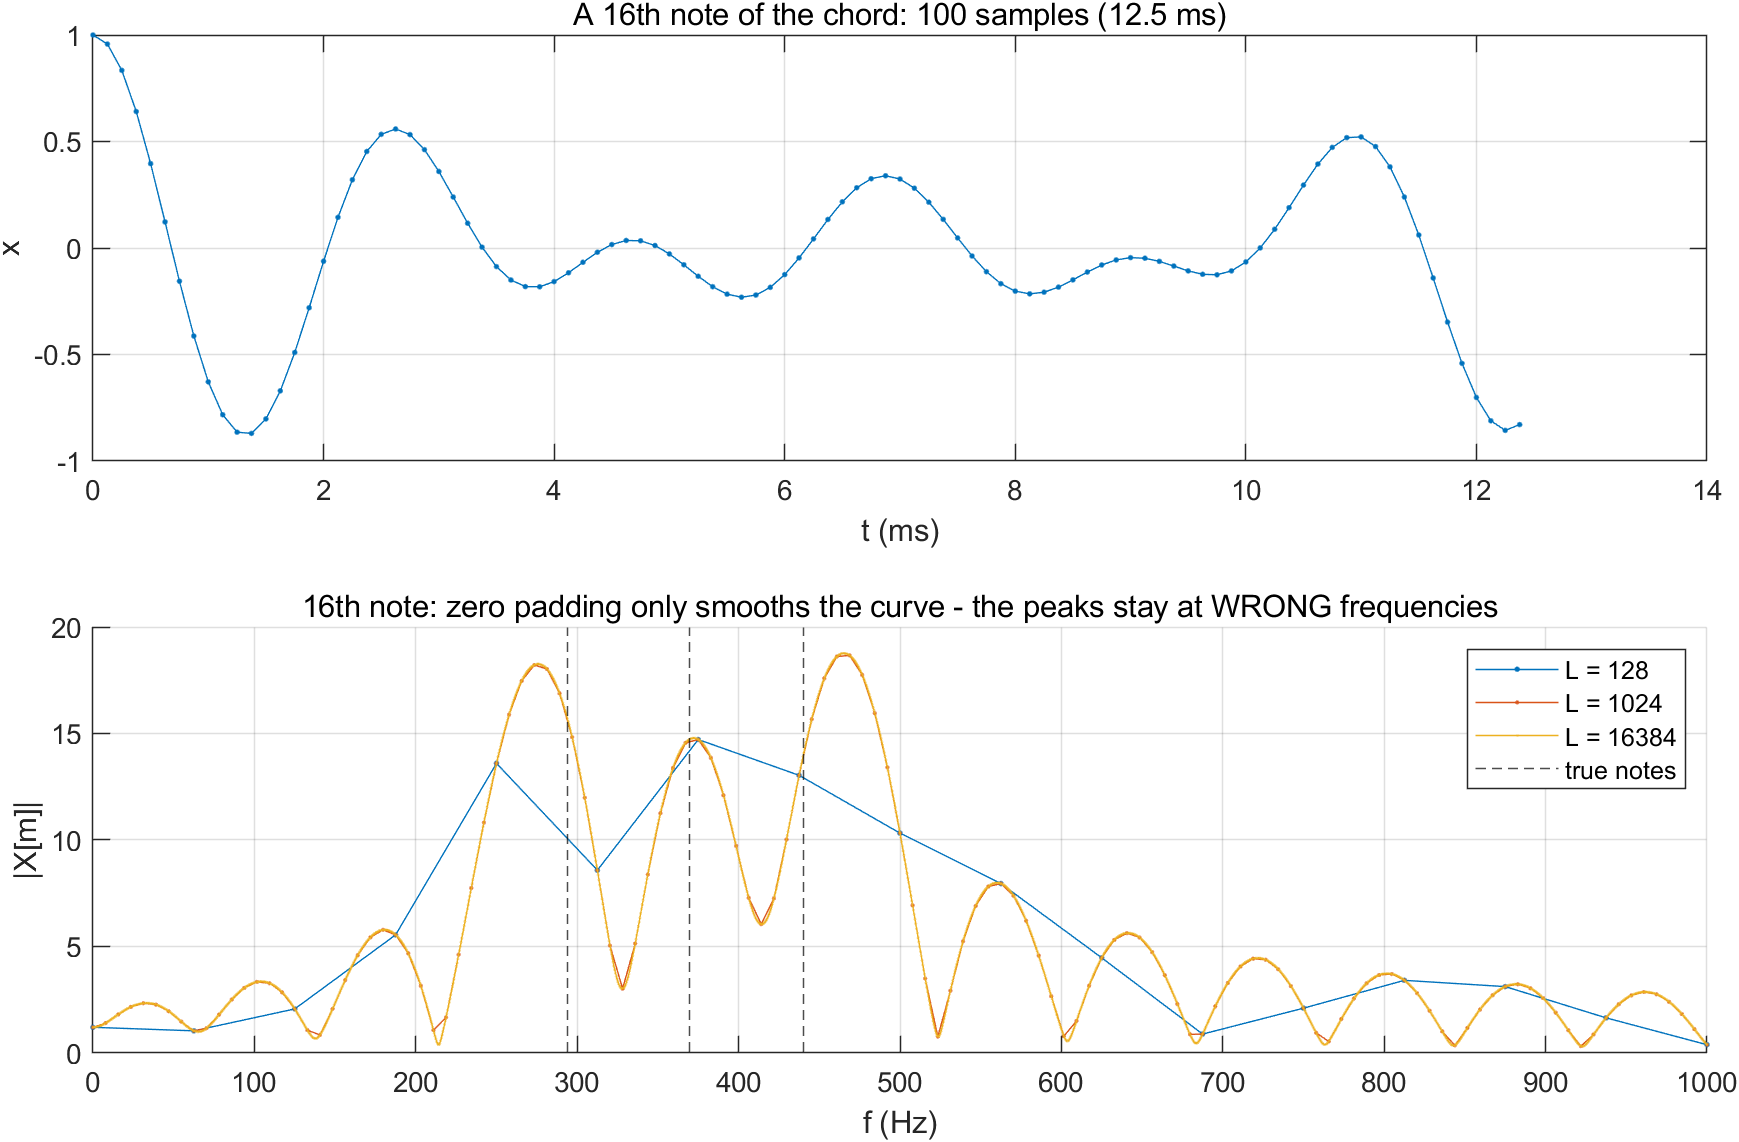
\includegraphics[width=0.82\textwidth]{Ex4_3_16th_zero_padding.png}
    \caption{One 16th note of the chord (100 samples) and its DFT with $L=128$, $1024$ and $16384$.}
    \label{fig:ex4-3}
\end{figure}

\begin{figure}[!htbp]
    \centering
    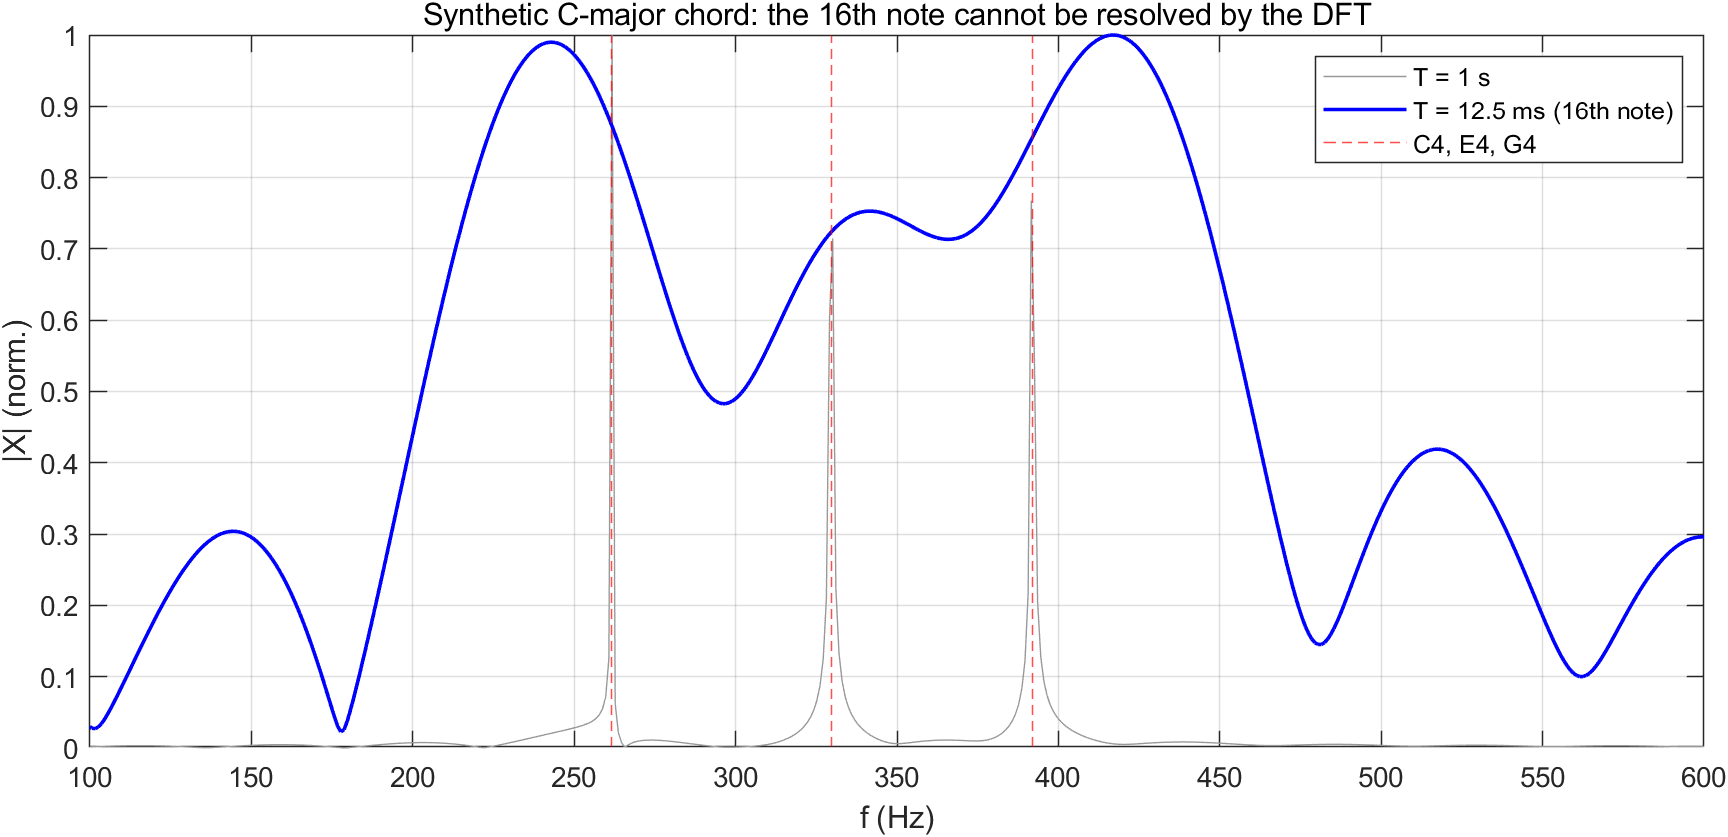
\includegraphics[width=0.82\textwidth]{Ex4_4_synthetic_C_chord.png}
    \caption{Synthesised C-major chord: 1 s record (grey) vs.\ 16th-note record (blue).}
    \label{fig:ex4-4}
\end{figure}

\begin{table}[!htbp]
\centering
\caption{Peaks found for different note durations (true chord: D4 F\#4 A4).}
\label{tab:ex4}
\small\setlength{\tabcolsep}{3pt}
\begin{tabular}{lrrll}
\toprule
Duration & $N$ & $f_s/N$ (Hz) & Rectangular: peaks (Hz) $\to$ notes & Hann: peaks (Hz) $\to$ notes\\
\midrule
1/16 note & 100  & 80 & 275, 372, 465 $\to$ C\#4 F\#4 A\#4 & 256, 475 $\to$ C4 A\#4\\
1/8 note  & 200  & 40 & 287, 373, 445 $\to$ D4 F\#4 A4      & 313, 421 $\to$ D\#4 G\#4\\
1/4 note  & 400  & 20 & 293, 371, 440 $\to$ D4 F\#4 A4      & 294, 370, 440 $\to$ D4 F\#4 A4\\
1/2 note  & 800  & 10 & 294, 370, 440 $\to$ D4 F\#4 A4      & 294, 370, 440 $\to$ D4 F\#4 A4\\
whole     & 1600 &  5 & 294, 370, 440 $\to$ D4 F\#4 A4      & 294, 370, 440 $\to$ D4 F\#4 A4\\
\bottomrule
\end{tabular}
\end{table}

\begin{table}[!htbp]
\centering
\caption{Least-squares note-grid fit using only one 16th note (100 samples).}
\label{tab:ex4-ls}
\begin{tabular}{lll}
\toprule
Test signal & Identified notes & Relative residual\\
\midrule
\texttt{hexian1} 16th note, clean            & D4 F\#4 A4 & $7.5\times10^{-9}$\\
\texttt{hexian1} 16th note + noise (SNR 20 dB) & D4 F\#4 A4 & $1.0\times10^{-2}$\\
Synthetic C4 E4 G4 16th note                 & C4 E4 G4   & $4.2\times10^{-9}$\\
\bottomrule
\end{tabular}
\end{table}

\subsection{Analysis of the Results}

\subsubsection{Composition of the Chord}
Figure~\ref{fig:ex4-1} shows three lines of equal height ($\approx0.33$) at \textbf{293.7 Hz (D4), 369.9 Hz (F\#4) and 439.9 Hz (A4)}, each within one cent of the equal-tempered values. The chord is therefore the \textbf{D major triad} D--F\#--A, i.e.\ 1--3--5 in D major, or 2--\#4--6 in the numbered notation of C major. Its frequency ratio $293.66:369.99:440\approx4:5:6$ is the typical ratio of a major triad. Because the three tones are not harmonically related within a short period, the waveform in the middle panel repeats only after a long time and looks irregular. Only the spectrum reveals its simple composition.

\subsubsection{The 16th-Note Problem}
The experiments confirm the theoretical analysis (Figure~\ref{fig:ex4-2}, Table~\ref{tab:ex4}):
\begin{itemize}
    \item \textbf{1/16 note (12.5 ms, $f_s/N=80$ Hz).} The rectangular window shows three bumps, but at 275, 372 and 465 Hz. These would be read as \textbf{C\#4, F\#4, A\#4}, two of the three notes being wrong by a semitone. The bumps are not true peaks: the three main lobes, each $\pm80$ Hz wide, overlap and interfere. The Hann window merges them into only two lumps (read as C4 and A\#4). Such a short note contains only 3.7 periods of D4, too few to define the frequencies.
    \item \textbf{1/8 note (25 ms, 40 Hz).} The rectangular window just separates the notes, with errors of 3--7 Hz. The Hann window, with its doubled main lobe, still fails.
    \item \textbf{1/4 note (50 ms) and longer.} Both windows give the correct chord, and the accuracy improves further with duration. The threshold lies between 14.3 ms and 28.6 ms, as predicted.
\end{itemize}
Figure~\ref{fig:ex4-3} shows that zero padding the 100 samples to $L=1024$ or $16384$ only smooths the curve: the bumps stay at the same wrong frequencies. The synthetic C-major chord (Figure~\ref{fig:ex4-4}) behaves in the same way. The limitation is therefore fundamental and not specific to this recording. In practice this means that a DFT-based transcription of fast passages (16th notes at this tempo) cannot identify the notes of a chord, whatever $L$ is chosen.

\subsubsection{Remedy: Using Prior Knowledge}
Table~\ref{tab:ex4-ls} shows that the least-squares fit on the note grid identifies the correct chord from the same 100 samples. For clean signals the residual is essentially zero ($10^{-9}$), and with 20 dB of added noise the result is still correct. The fit works because it does not rely on the resolution of the DFT. It assumes the signal consists of exactly three tones from a known set of frequencies, and a short record is enough to tell which set fits best. Its limitations are that the number of notes and the tuning must be known, and the cost grows quickly with the number of candidate notes.

% =====================================================================
\section{Topic 5: Spectral Analysis of a Scale with Harmonics}

\subsection{Analysis of the Simulation Task}

Each note of \texttt{yueyin2.wav} is modelled as
\begin{equation}
    x(t)=\sum_{n=1}^{M}A_n\cos(2\pi nf_0t+\varphi_n),
\end{equation}
so its spectrum is a ``ladder'' of lines at $f_0,2f_0,3f_0,\dots$. The whole record is a sequence of such notes.

\textbf{Can the composition be read directly from the whole-record spectrum?} No, for three reasons:
\begin{enumerate}
    \item \textbf{No time information.} The DFT of the whole record lists all lines of all notes together. Nothing tells us which line belongs to which note.
    \item \textbf{Harmonics coincide.} In equal temperament some intervals are (almost) simple integer ratios: the octave is exactly $2{:}1$ and the fifth is $2^{7/12}\approx1.498\approx3{:}2$. Hence $2f_{\mathrm{C4}}=f_{\mathrm{C5}}=523.25$ Hz, $3f_{\mathrm{C4}}=784.9\approx2f_{\mathrm{G4}}=784.0$ Hz, and $4f_{\mathrm{C4}}=2f_{\mathrm{C5}}\approx3f_{\mathrm{F4}}$. Lines closer than the line width of a 0.5 s note ($\approx4$ Hz) merge into one.
    \item \textbf{Heights are sums.} A shared line contains the contributions of several notes. Its height is therefore not the amplitude of any single harmonic.
\end{enumerate}

\textbf{Proposed method: time-segmented harmonic analysis.}
\begin{enumerate}
    \item \emph{Segmentation.} Split the signal into notes with the same pitch-change and energy-minimum procedure as in Topic 3.
    \item \emph{Per-note DFT.} Apply a Hann window $w$ and a 16384-point DFT to each note, and calibrate the amplitude as $\hat A(f)=2|X_w(f)|/\sum_kw[k]$.
    \item \emph{Fundamental.} $f_0$ is the lowest peak above 25\% of the strongest one, refined by parabolic interpolation. The lowest strong peak is used rather than the strongest, because a harmonic could be stronger than the fundamental.
    \item \emph{Harmonics.} Read $A_n$ as the maximum within $\pm2\%$ of $nf_0$, for all $nf_0<f_s/2$.
\end{enumerate}

\textbf{Verification.} We check the method in three independent ways:
\begin{itemize}
    \item \textbf{C1 (consistency):} from the per-note results, predict the height of every line of the whole-record spectrum, including the shared lines, and compare.
    \item \textbf{C2 (resynthesis):} rebuild the signal from the estimated $f_0$, $A_n$ and the measured envelope of each note, and compare waveform and spectrum with the original.
    \item \textbf{C3 (ground truth):} analyse a synthesised G-major scale with known harmonics $A_n=[1,0.6,0.35,0.15,0.05]$, unequal note lengths, an ADSR envelope and 30 dB noise, using exactly the same code.
\end{itemize}

\subsection{Simulation Code}

\begin{lstlisting}[caption={Topic 5: per-note harmonic analysis and verification (excerpt of \texttt{ex5\_harmonic.m})}]
[x, fs] = audioread('yueyin2.wav');
seg = segmentNotes(x, fs);                    % notes in time
for k = 1:size(seg, 1)
    xs = x(seg(k,1):seg(k,2));   w = hann(numel(xs));
    Xc = fft(xs .* w, 16384);
    Xm = abs(Xc(1:8192)) * 2 / sum(w);        % calibrated amplitude
    fAx = (0:8191).' * fs / 16384;
    % fundamental = lowest peak above 25 % of the maximum
    [~, pl] = findpeaks(Xm, 'MinPeakHeight', 0.25*max(Xm), ...
                        'MinPeakDistance', round(20/(fs/16384)));
    f0 = refinePeak(Xm, pl(1)) * fs / 16384;
    for n = 1:floor((fs/2 - 50)/f0)           % harmonic amplitudes
        band = abs(fAx - n*f0) <= 0.02*f0;
        A(n) = max(Xm(band));
    end
end

% C2: resynthesis with the estimated f0, A_n and the note envelope
env  = sqrt(movmean(xs.^2, round(2*fs/f0))) * sqrt(2);
env  = env / (sum(w.*env) / sum(w));          % match DFT amplitude
tone = cos(2*pi*tk*(1:M)*f0 + phi) * A.';     % sum of harmonics
xr(idx) = tone .* env;
\end{lstlisting}

\subsection{Simulation Results}

\begin{figure}[!htbp]
    \centering
    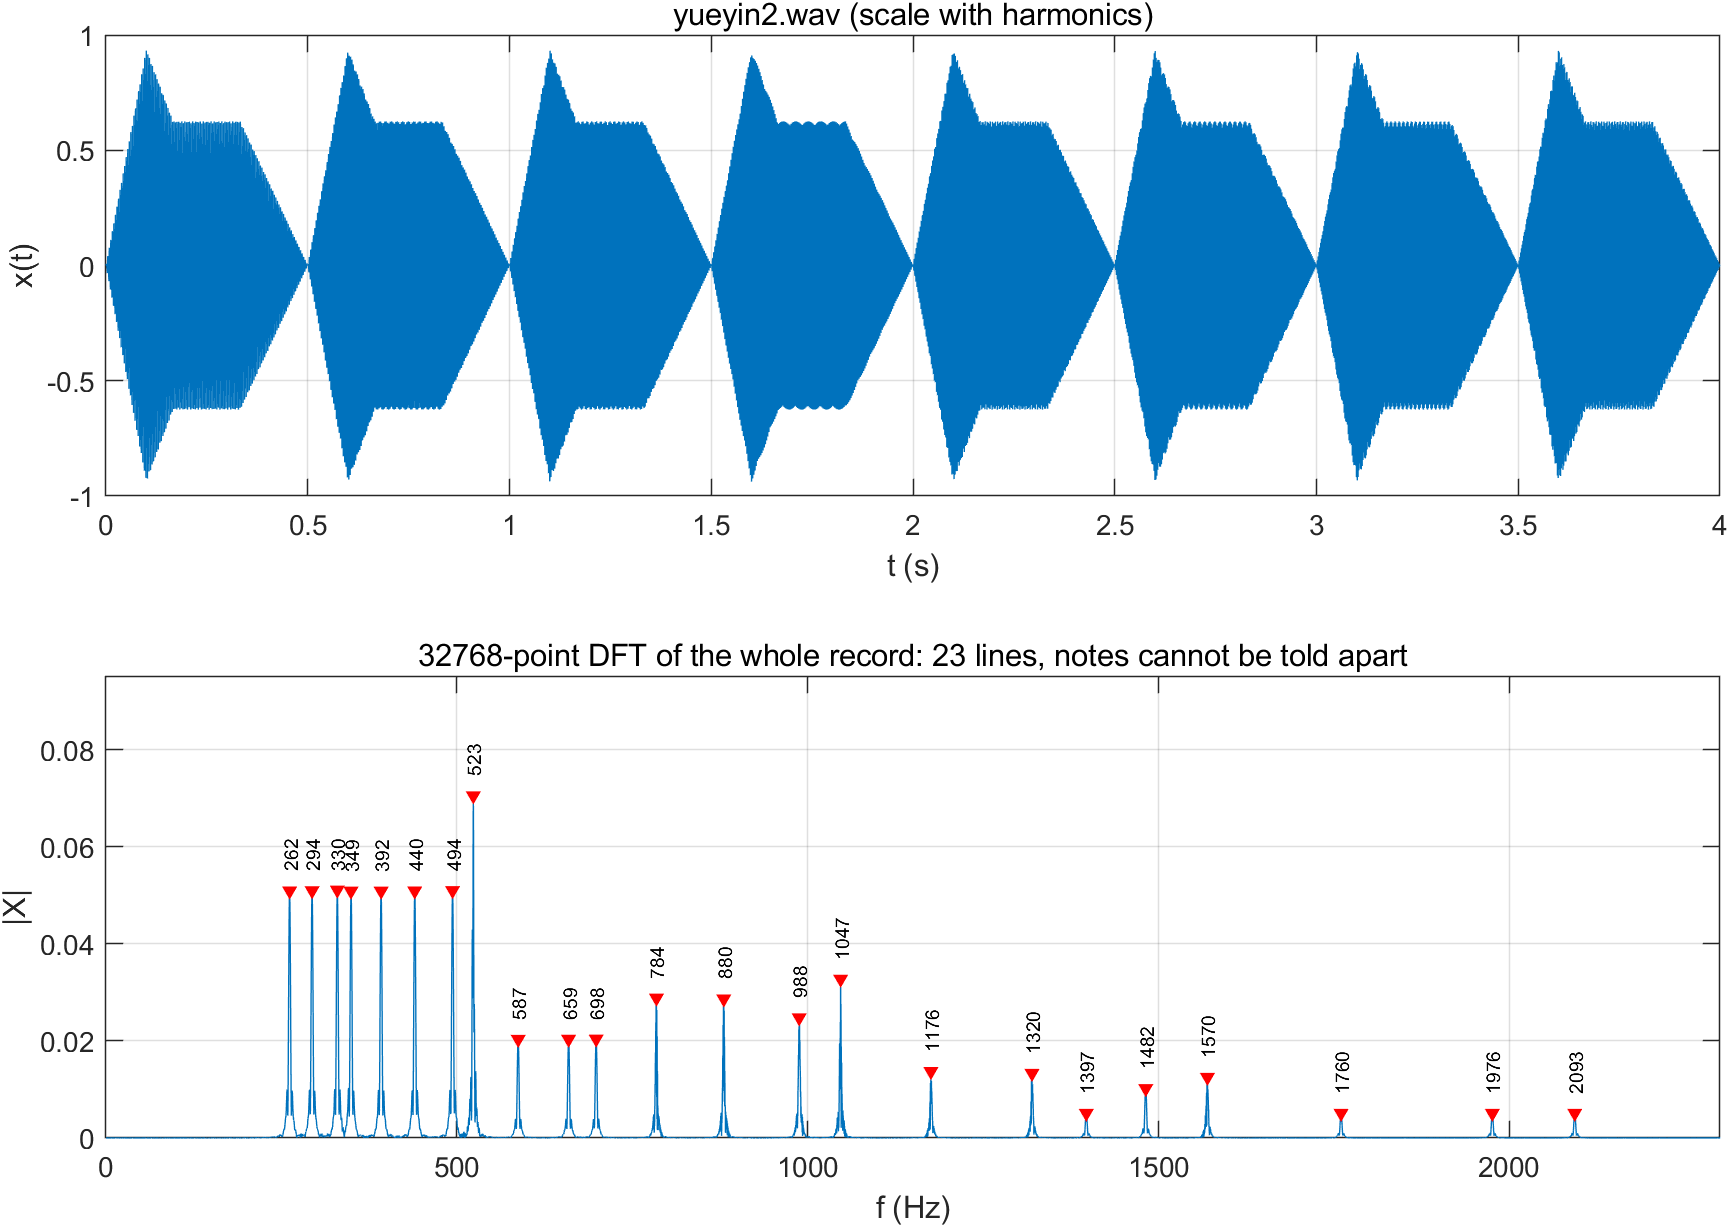
\includegraphics[width=1\textwidth]{Ex5_1_whole_spectrum.png}
    \caption{\texttt{yueyin2.wav} and the DFT of the whole record: 23 spectral lines between 261 and 2093 Hz.}
    \label{fig:ex5-1}
\end{figure}

\begin{figure}[!htbp]
    \centering
    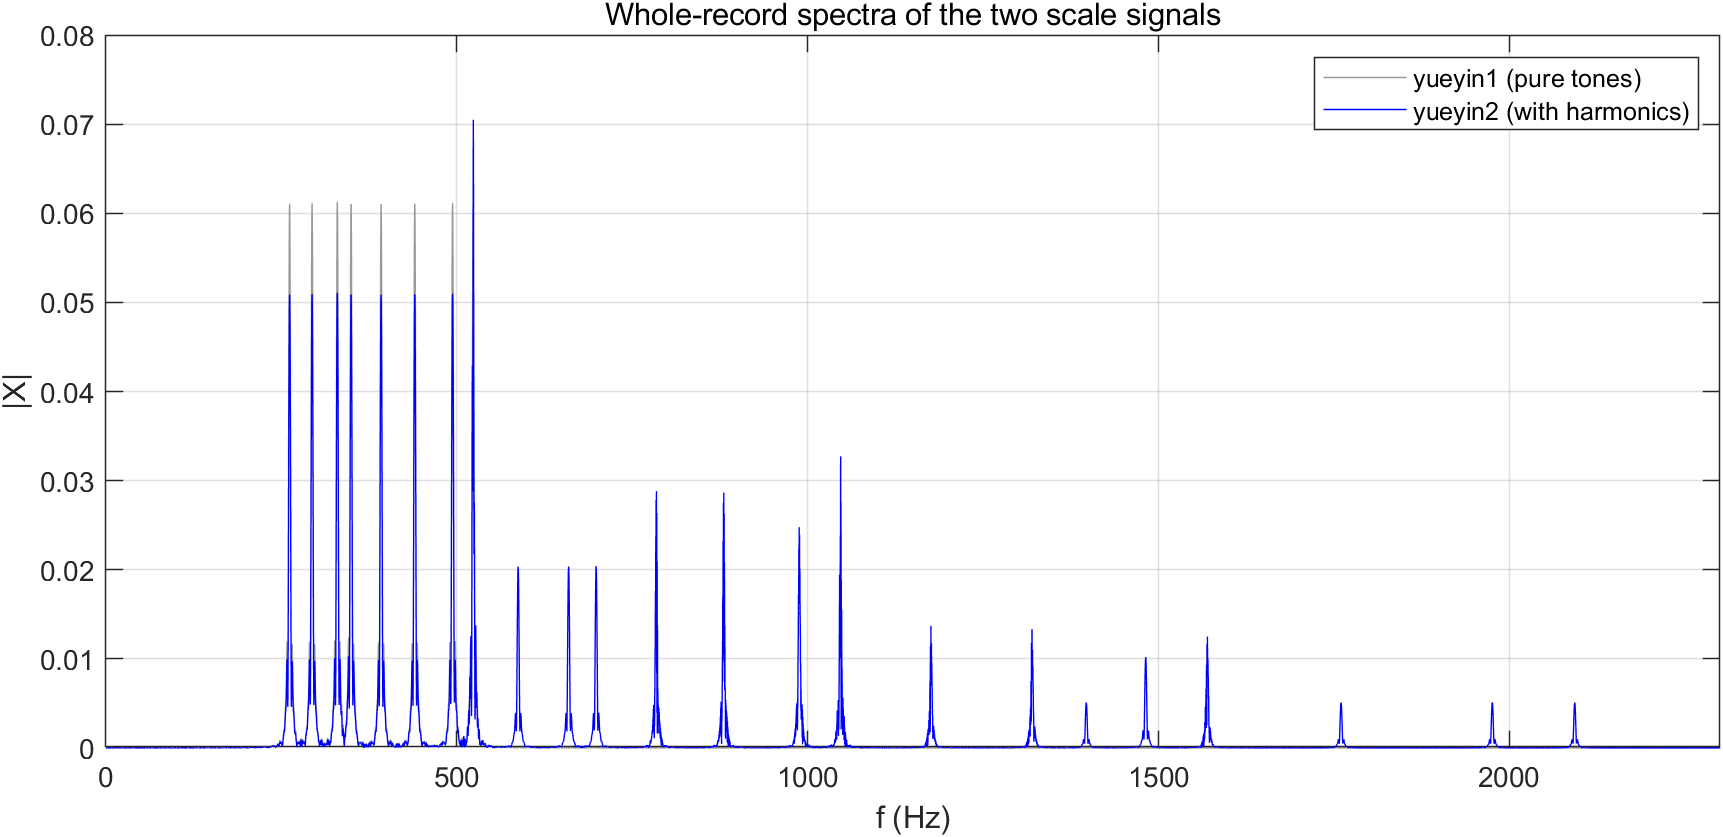
\includegraphics[width=1\textwidth]{Ex5_2_compare_yueyin1_2.png}
    \caption{Whole-record spectra of \texttt{yueyin1} (pure tones, grey) and \texttt{yueyin2} (with harmonics, blue).}
    \label{fig:ex5-2}
\end{figure}

\begin{figure}[!htbp]
    \centering
    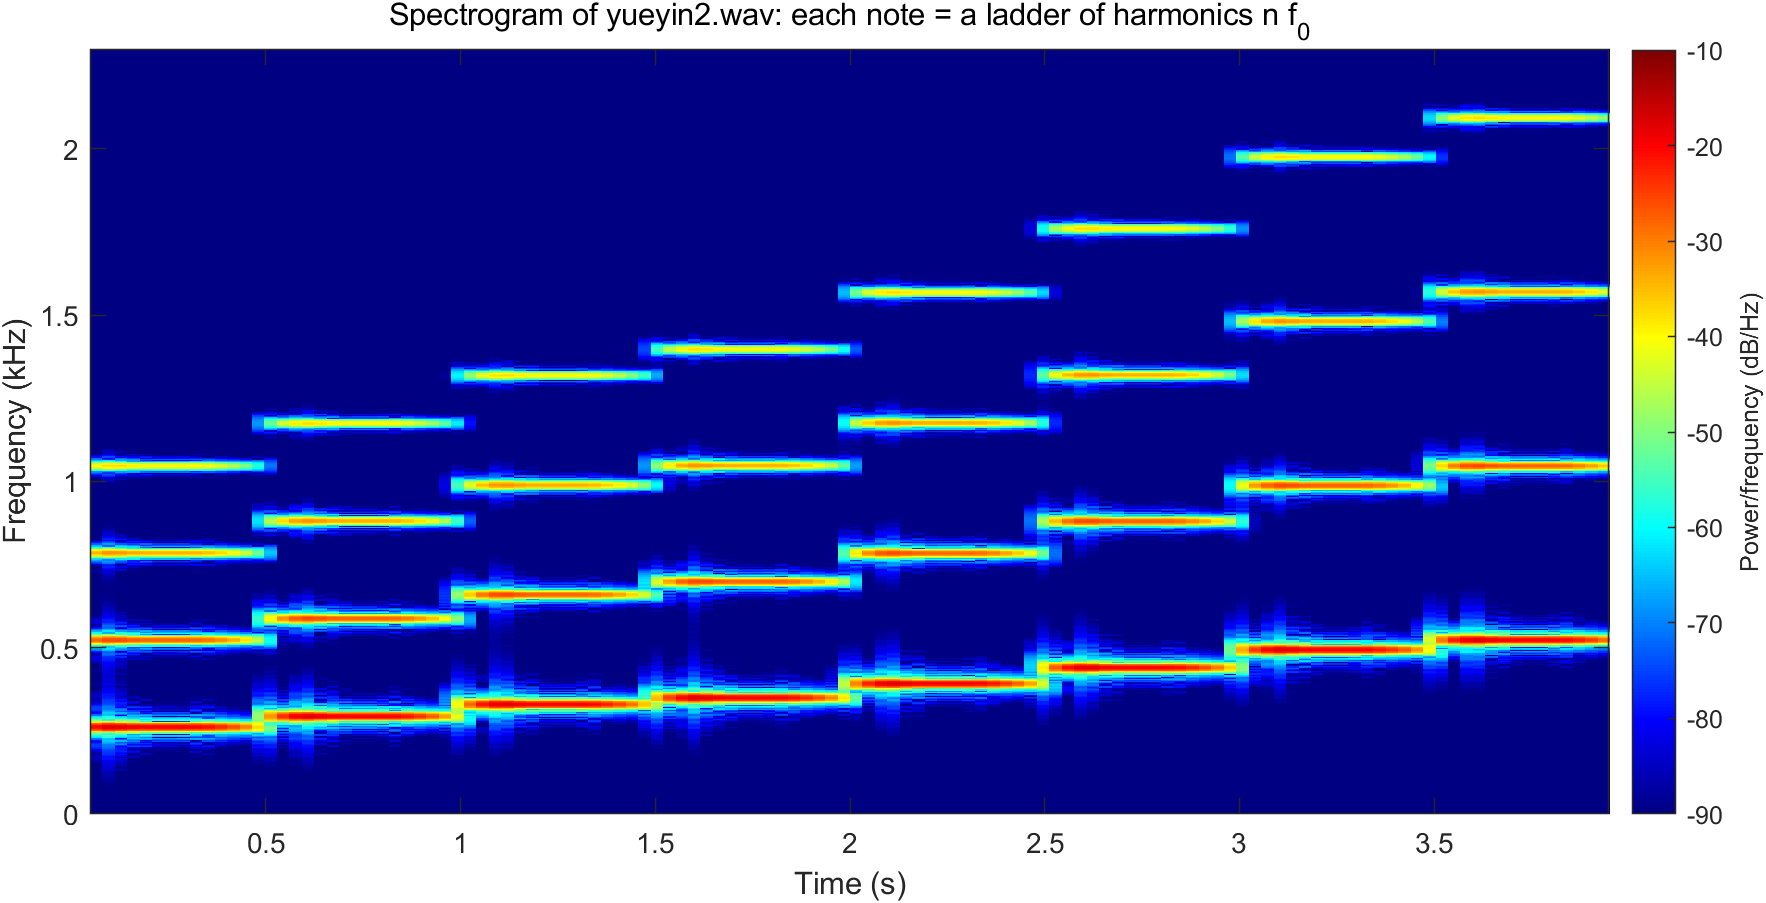
\includegraphics[width=1\textwidth]{Ex5_3_spectrogram.png}
    \caption{Spectrogram of \texttt{yueyin2.wav}: each note appears as a ladder of harmonics $nf_0$.}
    \label{fig:ex5-3}
\end{figure}

\begin{figure}[!htbp]
    \centering
    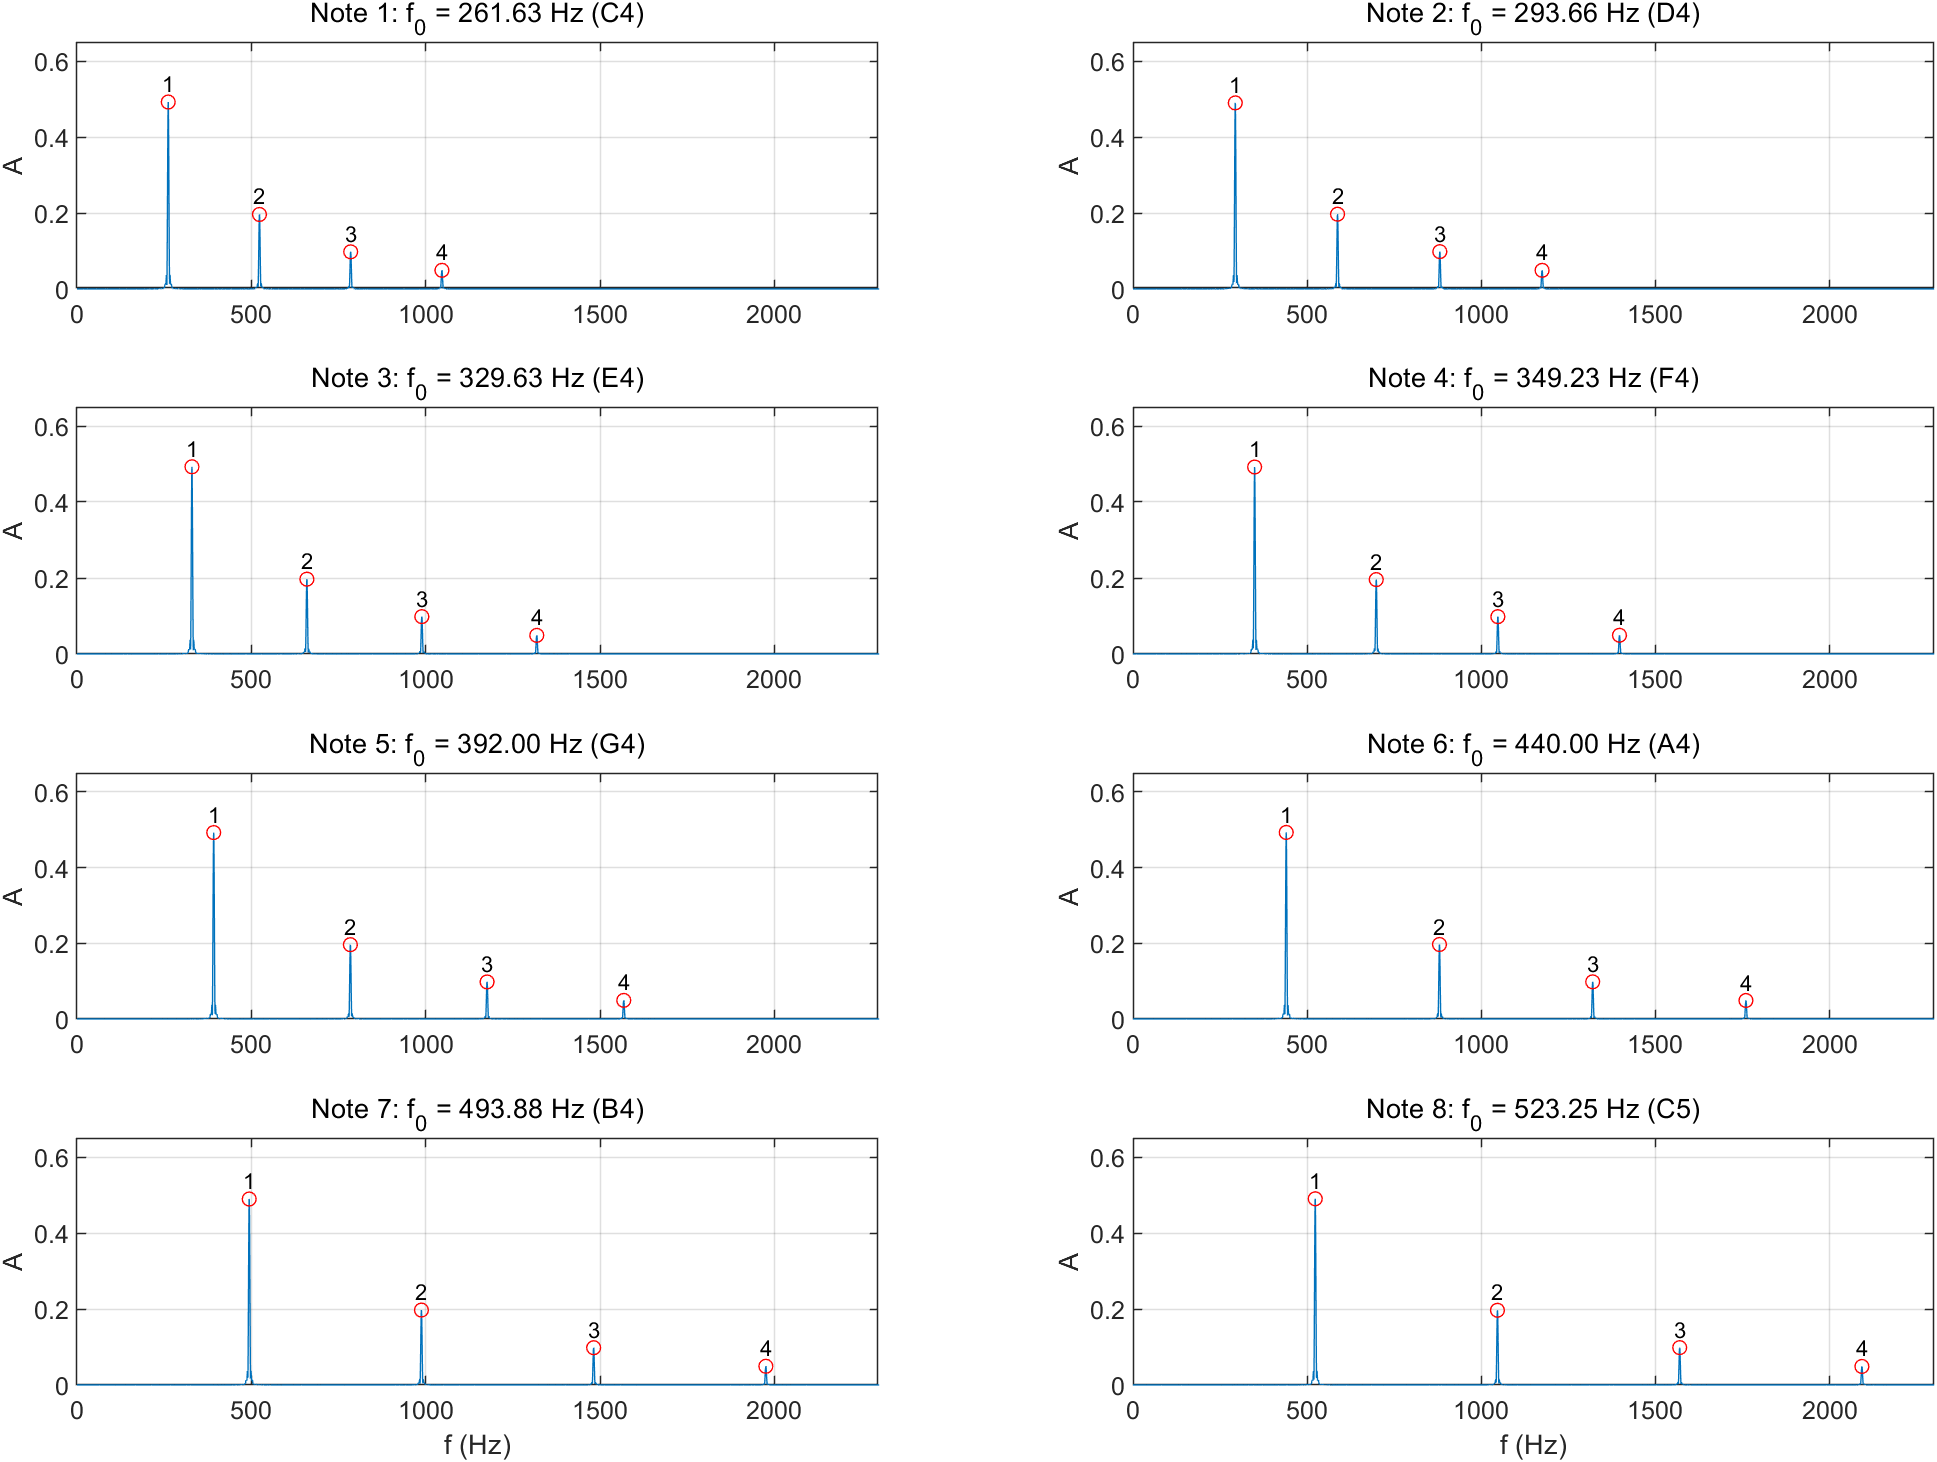
\includegraphics[width=1\textwidth]{Ex5_4_per_note_spectra.png}
    \caption{Calibrated amplitude spectrum of every note with the detected harmonics (red circles, harmonic number above).}
    \label{fig:ex5-4}
\end{figure}

\begin{figure}[!htbp]
    \centering
    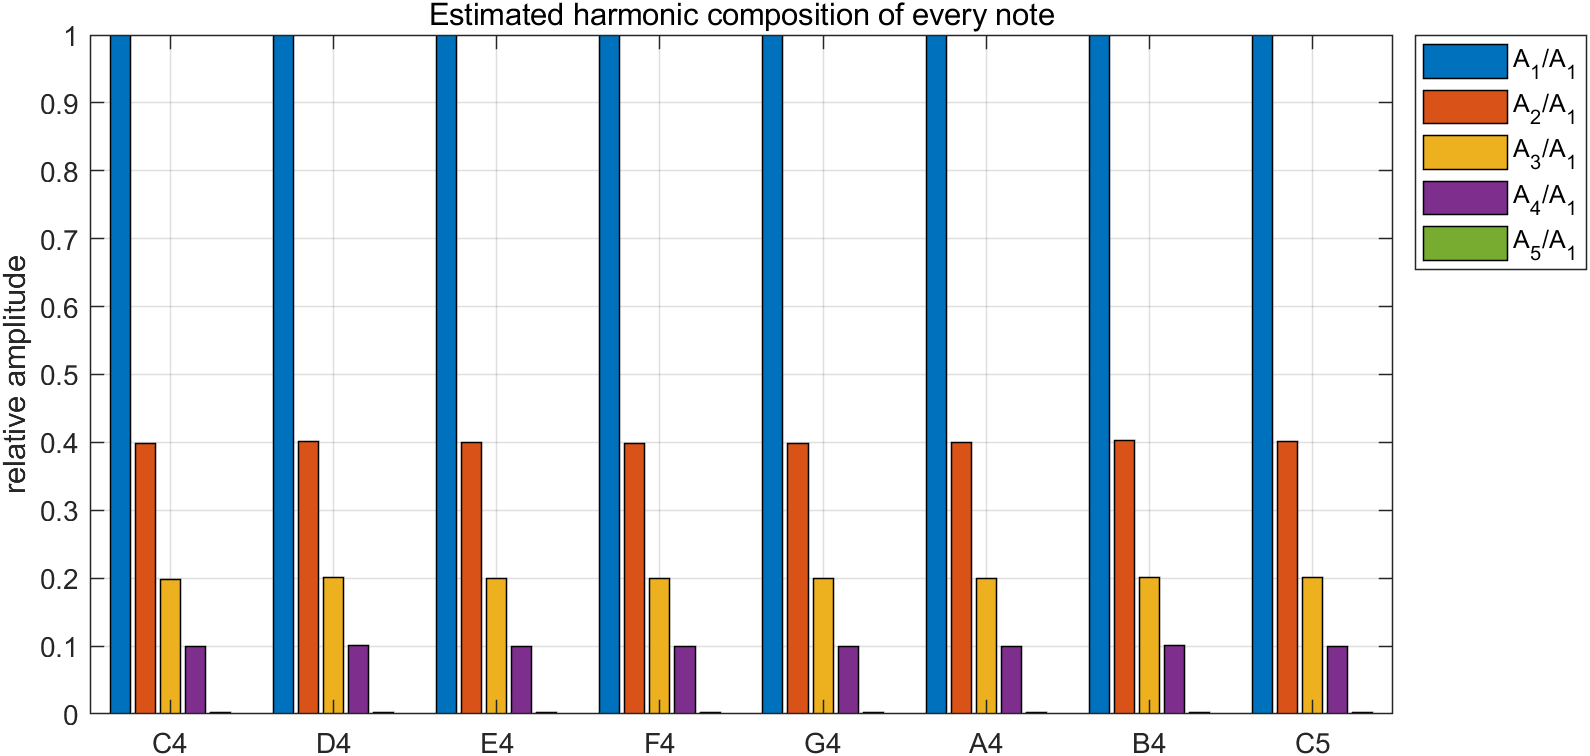
\includegraphics[width=0.8\textwidth]{Ex5_5_harmonic_amplitudes.png}
    \caption{Estimated relative harmonic amplitudes $A_n/A_1$ of the eight notes.}
    \label{fig:ex5-5}
\end{figure}

\begin{table}[!htbp]
\centering
\caption{Spectral composition of every note of \texttt{yueyin2.wav}.}
\label{tab:ex5}
\small\setlength{\tabcolsep}{4pt}
\begin{tabular}{clcccccl}
\toprule
Note & Name & $f_0$ (Hz) & $A_1$ & $A_2/A_1$ & $A_3/A_1$ & $A_4/A_1$ & Harmonics (Hz)\\
\midrule
1 & C4 & 261.63 & 0.492 & 0.399 & 0.199 & 0.100 & 261.6, 523.3, 784.9, 1046.5\\
2 & D4 & 293.66 & 0.490 & 0.402 & 0.201 & 0.100 & 293.7, 587.3, 881.0, 1174.6\\
3 & E4 & 329.63 & 0.493 & 0.400 & 0.200 & 0.100 & 329.6, 659.3, 988.9, 1318.5\\
4 & F4 & 349.23 & 0.492 & 0.398 & 0.200 & 0.100 & 349.2, 698.5, 1047.7, 1396.9\\
5 & G4 & 392.00 & 0.493 & 0.399 & 0.199 & 0.100 & 392.0, 784.0, 1176.0, 1568.0\\
6 & A4 & 440.00 & 0.493 & 0.399 & 0.199 & 0.099 & 440.0, 880.0, 1320.0, 1760.0\\
7 & B4 & 493.88 & 0.489 & 0.403 & 0.200 & 0.101 & 493.9, 987.8, 1481.6, 1975.5\\
8 & C5 & 523.25 & 0.490 & 0.401 & 0.201 & 0.100 & 523.3, 1046.5, 1569.8, 2093.0\\
\bottomrule
\end{tabular}
\end{table}

\begin{table}[!htbp]
\centering
\caption{C1: shared lines of the whole-record spectrum, measured vs.\ predicted from the per-note results.}
\label{tab:ex5-c1}
\begin{tabular}{rccl}
\toprule
$f$ (Hz) & Measured & Predicted & Contributions (note $\times$ harmonic)\\
\midrule
 523.4 & 0.0705 & 0.0711 & C4$\times$2 + C5$\times$1\\
 784.4 & 0.0288 & 0.0305 & C4$\times$3 + G4$\times$2\\
 880.4 & 0.0287 & 0.0306 & D4$\times$3 + A4$\times$2\\
 987.8 & 0.0248 & 0.0306 & E4$\times$3 + B4$\times$2\\
1046.9 & 0.0327 & 0.0356 & C4$\times$4 + F4$\times$3 + C5$\times$2\\
1175.5 & 0.0137 & 0.0152 & D4$\times$4 + G4$\times$3\\
1319.6 & 0.0133 & 0.0153 & E4$\times$4 + A4$\times$3\\
1569.6 & 0.0125 & 0.0153 & G4$\times$4 + C5$\times$3\\
\midrule
\multicolumn{4}{l}{All 23 lines: mean $|$relative error$|$ = 3.7\%; unshared lines agree within 1\%.}\\
\bottomrule
\end{tabular}
\end{table}

\begin{figure}[!htbp]
    \centering
    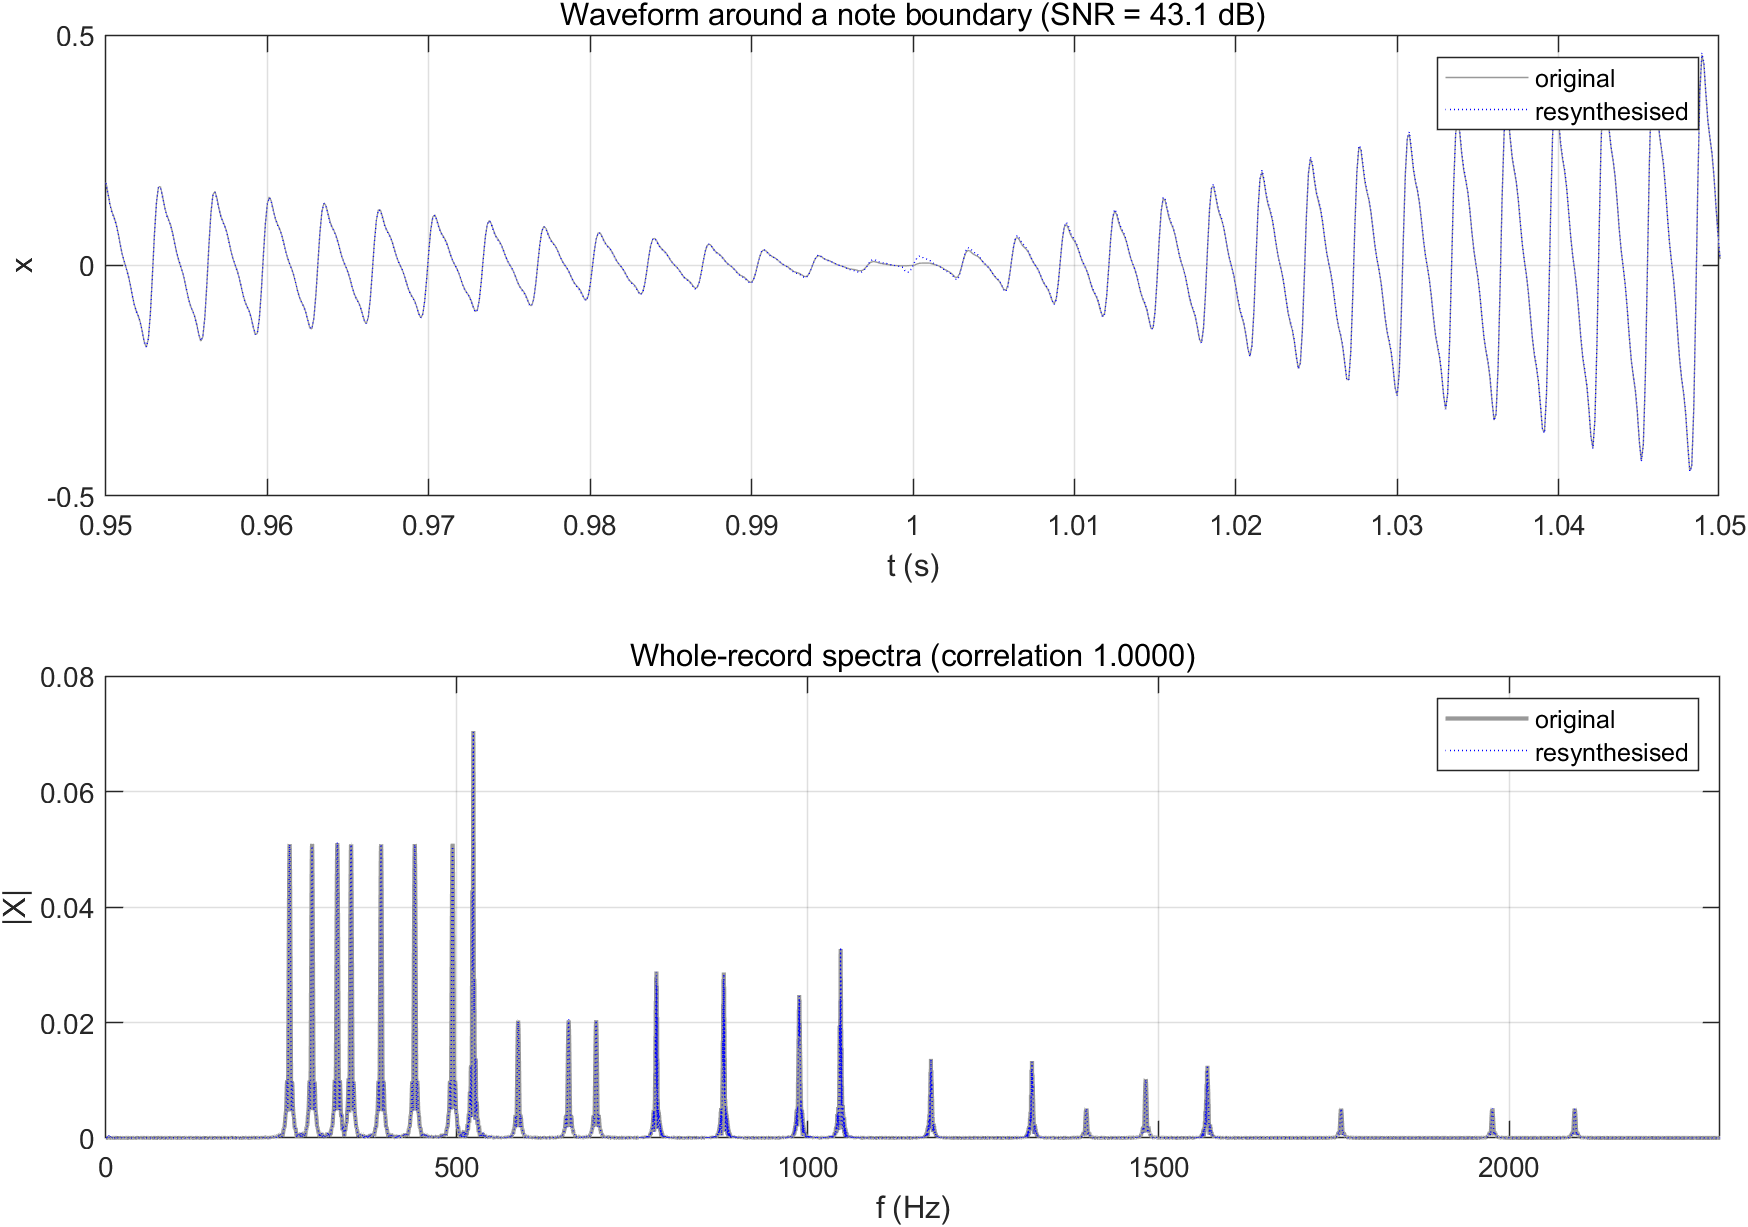
\includegraphics[width=0.85\textwidth]{Ex5_6_resynthesis.png}
    \caption{C2: original vs.\ resynthesised signal, waveform around a note boundary (top) and whole-record spectra (bottom).}
    \label{fig:ex5-6}
\end{figure}

\begin{figure}[!htbp]
    \centering
    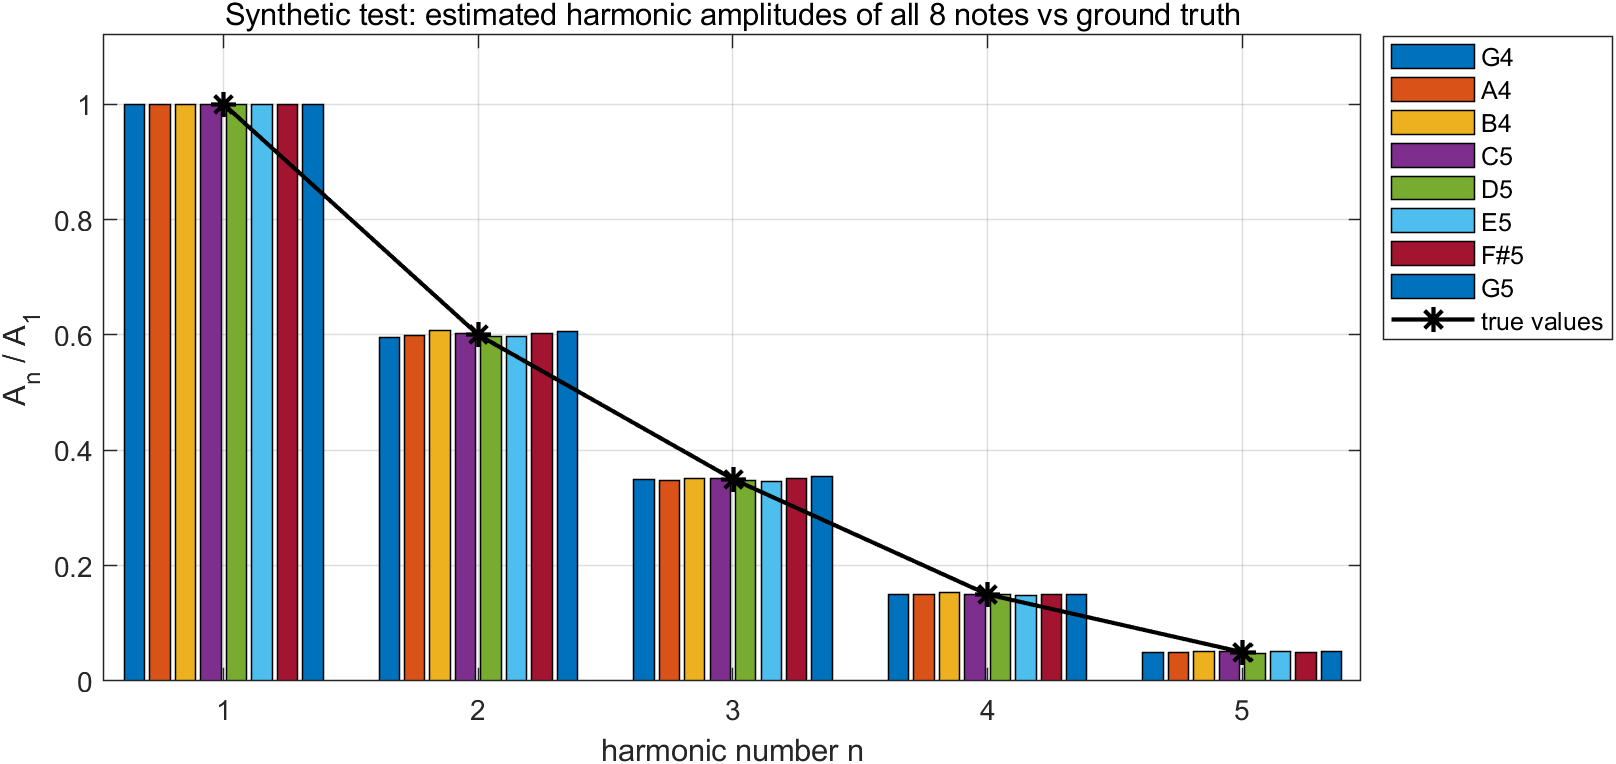
\includegraphics[width=0.82\textwidth]{Ex5_7_synthetic_test.png}
    \caption{C3: estimated $A_n/A_1$ of all eight notes of the synthetic G-major scale vs.\ the true values (black).}
    \label{fig:ex5-7}
\end{figure}

\subsection{Analysis of the Results}

\subsubsection{Why the Whole-Record Spectrum Is Not Enough}
Compared with \texttt{yueyin1} (Figure~\ref{fig:ex5-2}), \texttt{yueyin2} contains 15 additional lines up to 2093 Hz, 23 in total (Figure~\ref{fig:ex5-1}). Read naively, the spectrum could suggest 23 different ``notes''. Checking every line against the scale shows that 11 of the 23 lines can come from more than one note: for example, 523 Hz could be C4$\times$2 or C5$\times$1, and 1047 Hz could be C4$\times$4, F4$\times$3 or C5$\times$2. The line heights are also misleading. The 523 Hz line is the highest in the whole spectrum ($1.38\times$ the other fundamentals), not because C5 is louder, but because the second harmonic of C4 adds to the fundamental of C5. The spectral composition of the individual notes therefore \textbf{cannot} be determined directly from the whole-record spectrum.

\subsubsection{Composition of Each Note}
After segmentation, every note shows a clean harmonic ladder (Figures~\ref{fig:ex5-3} and~\ref{fig:ex5-4}). The results in Table~\ref{tab:ex5} and Figure~\ref{fig:ex5-5} are strikingly regular:
\begin{itemize}
    \item The fundamentals are exactly the eight notes of the C major scale, C4--C5, as in Topic 3. \texttt{yueyin2} is the same scale played with a richer timbre.
    \item Every note contains exactly \textbf{four harmonics}. Harmonics $n\ge5$ are below 1\% of $A_1$.
    \item The relative amplitudes are the same for all notes: $A_1:A_2:A_3:A_4=1:0.40:0.20:0.10$ (absolute $\approx0.49:0.20:0.10:0.05$), with a spread of less than $\pm0.003$.
\end{itemize}
Each note can thus be written as $x(t)\approx0.49\,[\cos(2\pi f_0t)+0.4\cos(4\pi f_0t)+0.2\cos(6\pi f_0t)+0.1\cos(8\pi f_0t)]$ under its attack/decay envelope.

\subsubsection{Verification}
\begin{itemize}
    \item \textbf{C1.} Using the per-note results, we predict all 23 line heights of the whole-record spectrum with a mean error of 3.7\%. Lines belonging to a single note agree within 1\%. Shared lines are slightly \emph{lower} than the plain sum of their contributions (Table~\ref{tab:ex5-c1}). The contributions come from different time intervals, so in the whole-record DFT they add as complex numbers with different phases, and $|\sum_i z_i|\le\sum_i|z_i|$. The largest deviation (987.8 Hz) occurs where the two contributions, E4$\times$3 at 988.9 Hz and B4$\times$2 at 987.8 Hz, are 1.1 Hz apart and partly cancel.
    \item \textbf{C2.} The signal resynthesised from 8 fundamentals, $8\times4$ amplitudes and the note envelopes coincides with the original (Figure~\ref{fig:ex5-6}): spectral correlation $\approx1.000$ and waveform SNR 43.1 dB. The resynthesised signal is saved as \texttt{yueyin2\_resynth.wav} for a listening comparison.
    \item \textbf{C3.} For the synthetic G-major scale (G4 to G5, including F\#5) all 8 notes are found, with pitch errors of at most 0.01 cent and amplitude errors $|\hat A_n/\hat A_1-A_n|\le0.008$ (Figure~\ref{fig:ex5-7}). This holds despite unequal note lengths, a different envelope and noise.
\end{itemize}
The three checks agree: segmenting the signal in time before applying the DFT is a reliable way to determine the spectral composition of every note. The price is coarser frequency resolution (each note lasts only 0.5 s), which, as Topic 4 showed, is not a problem as long as the notes are not too short.

% =====================================================================
\section{Problems Encountered and Solutions}

\begin{enumerate}
    \item \textbf{Zero padding looks like better resolution (Topic 2).} With $L=512$ the curve looks smooth and ``high-resolution'', but it still has one peak. \emph{Solution:} distinguish the bin spacing $2\pi/L$ from the physical resolution $2\pi/N$, and increase $N$ instead.
    \item \textbf{Spurious peaks (Topics 2 and 4).} With tapered windows at $N=128$ and with the 16th-note chord, the DFT shows the expected number of peaks but at wrong frequencies. \emph{Solution:} always compare the line spacing with the theoretical resolution of the window, and check peak positions, not only their number.
    \item \textbf{Notes too short for the DFT (Topic 4).} \emph{Solution:} a parametric least-squares fit on the equal-tempered note grid. It recovers the chord from 100 samples, even with noise.
    \item \textbf{Overlapping harmonics (Topic 5).} \emph{Solution:} short-time segmentation followed by a per-note DFT, verified by line-height prediction, resynthesis and a ground-truth test.
    \item \textbf{Inaccurate note boundaries.} The first version of the segmentation placed the boundaries up to 20 ms too late, because it works on 64 ms frames. \emph{Solution:} refine every boundary to the short-time energy minimum within $\pm40$ ms. The boundaries then fall within 1 ms of the true 0.5 s grid.
    \item \textbf{Poor first resynthesis (Topic 5).} Our first resynthesis reached only 8.1 dB SNR. The phases were read from a single DFT bin, and the envelope was scaled by its maximum instead of its Hann-weighted mean. \emph{Solution:} normalise the envelope by $\sum_k w[k]\,e[k]/\sum_kw[k]$, which is exactly the factor contained in the DFT amplitude, and obtain the phases by a least-squares fit. The SNR improved to 43.1 dB.
\end{enumerate}

% =====================================================================
\section{Self-Study Content}

Beyond the lecture material, we studied the following topics for this seminar:
\begin{itemize}
    \item The equal-tempered scale, MIDI note numbers and cents, used to convert measured frequencies to note names, and the structure of major scales and triads (interval patterns 2-2-1-2-2-2-1 and 4:5:6).
    \item Window functions and their main-lobe/side-lobe trade-off \cite{harris}, and the conditions for leakage-free (coherent) sampling.
    \item The short-time Fourier transform and spectrograms for signals whose spectrum changes with time \cite{oppenheim}.
    \item Parabolic interpolation of spectral peaks for sub-bin frequency estimation \cite{smith}, and amplitude calibration of windowed DFTs.
    \item Parametric (model-based) spectral estimation, in particular least-squares fitting of sinusoids, which is not limited by the $1/T$ resolution of the DFT \cite{stoica}.
    \item Harmonic analysis/resynthesis of musical tones, and the MATLAB functions \texttt{fft}, \texttt{findpeaks}, \texttt{spectrogram}, \texttt{audioread} and \texttt{audiowrite} \cite{matlab}.
\end{itemize}

% =====================================================================
\begin{thebibliography}{9}
\addcontentsline{toc}{section}{References}

\bibitem{chen} Chen Houjin, Hu Jian, Xue Jian, \emph{Signals and Systems}, 2nd ed. Beijing: Tsinghua University Press / Beijing Jiaotong University Press, pp.~222--223.

\bibitem{oppenheim} A.~V. Oppenheim and R.~W. Schafer, \emph{Discrete-Time Signal Processing}, 3rd ed. Upper Saddle River, NJ: Pearson, 2010.

\bibitem{proakis} J.~G. Proakis and D.~G. Manolakis, \emph{Digital Signal Processing: Principles, Algorithms, and Applications}, 4th ed. Upper Saddle River, NJ: Pearson, 2007.

\bibitem{harris} F.~J. Harris, ``On the use of windows for harmonic analysis with the discrete Fourier transform,'' \emph{Proceedings of the IEEE}, vol.~66, no.~1, pp.~51--83, 1978.

\bibitem{stoica} P.~Stoica and R.~L. Moses, \emph{Spectral Analysis of Signals}. Upper Saddle River, NJ: Prentice Hall, 2005.

\bibitem{smith} J.~O. Smith III, \emph{Spectral Audio Signal Processing}. W3K Publishing, 2011 (Chapter ``Quadratic Interpolation of Spectral Peaks'').

\bibitem{matlab} The MathWorks, Inc., \emph{MATLAB R2024b Documentation: fft, findpeaks, spectrogram}. Natick, MA, 2024.

\end{thebibliography}

% =====================================================================
\appendix
\section{Complete MATLAB Source Code}

All scripts are run together by \texttt{run\_all.m}. Each script reads the audio files from its own folder and saves its figures to \texttt{figures/}. Explanatory comments are shortened here; the submitted \texttt{.m} files contain the full comments.

\lstset{basicstyle=\ttfamily\scriptsize\setstretch{1.0}, numberstyle=\tiny\color{gray}, aboveskip=6pt, belowskip=4pt}
\lstinputlisting[caption={\texttt{run\_all.m}}]{code/run_all.m}
\lstinputlisting[caption={\texttt{ex2\_resolution.m} (Topic 2)}]{code/ex2_resolution.m}
\lstinputlisting[caption={\texttt{ex3\_scale.m} (Topic 3)}]{code/ex3_scale.m}
\lstinputlisting[caption={\texttt{ex4\_chord.m} (Topic 4)}]{code/ex4_chord.m}
\lstinputlisting[caption={\texttt{ex5\_harmonic.m} (Topic 5)}]{code/ex5_harmonic.m}

\end{document}
